% Author:  Brad Burkman
% Date:  21 August 2018
% Notes for Fall 2018 CSCE 515
%	Principles of Computer Graphics
%	Dr. Christoph Borst

\documentclass[12pt]{article}
\usepackage{tikz}
\usetikzlibrary{arrows, intersections, calc}
\usepackage{pgfmath}
\usepackage{tikz-3dplot}
\usepackage{setspace}
\usepackage{amsmath}
\usepackage{array}
\usepackage{hyperref}
\usepackage{verbatim}
%\usepackage{color}
\setlength{\pdfpageheight}{11in}
\setlength{\textheight}{9in}
\setlength{\voffset}{-1in}
\setlength{\oddsidemargin}{0pt}
\setlength{\marginparsep}{0pt}
\setlength{\marginparwidth}{0pt}
\setlength{\marginparpush}{0pt}
\setlength{\textwidth}{6.5in}

\usepackage{listings}
\usepackage{xcolor} % for setting colors

% set the default code style
\lstset{
    frame=tb, % draw a frame at the top and bottom of the code block
    tabsize=4, % tab space width
    showstringspaces=false, % don't mark spaces in strings
    numbers=left, % display line numbers on the left
    commentstyle=\color{green}, % comment color
    keywordstyle=\color{blue}, % keyword color
    stringstyle=\color{red} % string color
}

\pagestyle{empty}
\begin{document}
\setlength{\parindent}{0pt}
\begin{spacing}{1.2}

Brad Burkman's Notes for

\qquad CSCE 515 Principles of Computer Graphics

\qquad Dr. Christoph Borst, CBDI co-PI, 
OLVR 342, 
\url{cbx99999@louisiana.edu}

\qquad Fall 2018

\url{bburkman@lsmsa.edu}

\url{C00412257@louisiana.edu}

\

Grader:  Jason Woodworth, \url{downtothelastpixel@gmail.com}

\tableofcontents

%%%%%%%%%%%%
\section{Tuesday 21 August:  Introduction}
%%%%%%%%%%%%%

Ray Tracing

OpenGL 3.3

\qquad Couldn't find a textbook that did both the math and OpenGL 3.3 well.  

Cross Product v/s Dot Product of Vectors

Start with how lines and triangles are rendered.  

Acknowledge sources I used in homework and projects.  

Exam will be hard.  

Lagniappe - Come to VR lab to do a project.  

\


%%%%%%%%%%%%
\section{Math Review:  Dot Product and Cross Product}
%%%%%%%%%%%%%

Example of Dot Product and Cross Product:

$\vec{u} = \langle 1,2,3 \rangle$

$\vec{v} = \langle 4,5,6 \rangle$

\

$\vec{u} \cdot \vec{v} = 1 \cdot 4 + 2 \cdot 5 + 3 \cdot 6 = 4 + 10 + 18 = 32$

\

$\displaystyle \vec{w} = \vec{u} \times \vec{v} = 
	\left|
	\begin{tabular}{*3{>{$}c<{$}}}
		\vec{i} & \vec{j} & \vec{k} \cr
		1 & 2 & 3 \cr
		4 & 5 & 6 \cr
	\end{tabular}
	\right|
\ = \
	\left|
	\begin{tabular}{cc}
		2 & 3 \cr
		5 & 6 \cr
	\end{tabular}
	\right|
	\vec{i}
\ - \	
	\left|
	\begin{tabular}{cc}
		1 & 3 \cr
		4 & 6 \cr
	\end{tabular}
	\right|
	\vec{j}
\ + \ 
	\left|
	\begin{tabular}{cc}
		1 & 2 \cr
		4 & 5 \cr
	\end{tabular}
	\right|
	\vec{k}
\ = \
	-3\vec{i} + 6 \vec{j} - 3 \vec{k}
\ = \
	\langle -3,6,-3 \rangle
$

\

Is the cross product commutative?

\

$\displaystyle\vec{v} \times \vec{u} = 
	\left|
	\begin{tabular}{*3{>{$}c<{$}}}
		\vec{i} & \vec{j} & \vec{k} \cr
		4 & 5 & 6 \cr
		1 & 2 & 3 \cr
	\end{tabular}
	\right|
\ = \
	\left|
	\begin{tabular}{cc}
		5 & 6 \cr
		2 & 3 \cr
	\end{tabular}
	\right|
	\vec{i}
\ - \	
	\left|
	\begin{tabular}{cc}
		4 & 6 \cr
		1 & 3 \cr
	\end{tabular}
	\right|
	\vec{j}
\ + \ 
	\left|
	\begin{tabular}{cc}
		4 & 5 \cr
		1 & 2 \cr
	\end{tabular}
	\right|
	\vec{k}
\ = \
	3\vec{i} - 6 \vec{j} + 3 \vec{k}
\ = \
	\langle 3,-6,3 \rangle
\ = \ -\vec{w}
$

\

No, it's anti-commutative, but that's okay.  The cross product gives a vector, $\vec{w}$, orthogonal to both $\vec{u}$ and $\vec{v}$, and a constant multiple of $\vec{w}$ is still orthogonal to both other vectors.  

\

The cross product is also not associative, but satisfies the Jacobi identity.

$$a \times (b \times c) + b \times (c \times a) + c \times (a \times b) = 0 \ \forall a, b, c \in V$$


%%%%%%%%%%%%%%%%
\section{Math Review:  Algebra}
%%%%%%%%%%%%%%%%%%

A {\bf group} is a set $S$ with an operation (``+'')  such that:

\qquad The set S is {\it closed} under the operation, meaning that if $a,b \in S$, then $a+b \in S$.

\qquad The operation is associative, meaning that if $a,b,c \in S$, then $a+(b+c) = (a+b)+c$.

\qquad The set $S$ contains a unit element (``0''), such that $a+0 = 0+a = a \ \forall \ a \in S.$

\qquad For every element $a \in S$, there is an inverse element, $-a$, such that $a+(-a) = -a + a = 0$.

If the operation is commutative, meaning $a+b = b+a \ \forall \ a, b, \in S$, then $S$ is called an {\bf Abelian group.}

\

A {\bf ring} is a set $R$ with two operations, $+$ and $\cdot$, such that:

\qquad The set $R$ is an Abelian group.  

\qquad The set $R$ is closed under multiplication.

\qquad Multiplication is associative.  

\qquad The distributive laws hold:

\qquad \qquad $a \cdot (b+c) = a \cdot b + a \cdot c$

\qquad \qquad $(b+c) \cdot a = b \cdot a + c \cdot a$

A ring with a multiplicative identity (``1'') is called a {\bf ring with unit}.

If the ring has the property that if $a\cdot b = 0$ then $a=0$ or $b=0$, it is called a {\bf domain}.

If multiplication is commutative, then the ring is called a {\bf commutative ring}.

If a domain is commutative, then it is called an {\bf integral domain}.

\

A {\bf field} is a commutative ring with unit element (``1'') such that every nonzero element has an inverse.  

\

Quaternions are not a field because multiplication of quaternions is not commutative; however, every nonzero quaternion has a multiplicative inverse, so they are called a {\bf division ring}.


%%%%%%%%%
\section{Math Review:  Quaternions}
%%%%%%%%%%%

Complex numbers, $a+bi$ where $a$ and $b$ are real numbers and $i = \sqrt{-1}$, are two-dimensional numbers.  Quaternions, $a + bi + cj + dk$, are four-dimensional numbers.  Just as you can think of complex numbers being two-dimensional vectors having the basis vectors $1 = \langle 1,0 \rangle$ and $i = \langle 0,1 \rangle$, you can think of quaternions as four-dimensional vectors having the basis vectors 
$1 = \langle 1,0,0,0 \rangle$, 
$i = \langle 0,1,0,0 \rangle$, 
$j = \langle 0,0,1,0 \rangle$, 
$k = \langle 0,0,0,1 \rangle$, 

\

While complex numbers have the basis elements 1 and $i$ with, $i^2 = -1$, quaternions have this multiplication scheme for their basis elements.  Note that $i^2 = j^2 = k^2 = ijk = -1$, but they are anti-commutative, with, for example, $ij = -ji$.

\

\hfil\begin{tabular}{*5{>{$}c<{$}|}}
	\times & 1 & i & j & k \cr \hline
	1 & 1 & i & j & k \cr \hline
	i & i & -1 & k & -j \cr \hline
	j & j & -k & -1 & i \cr \hline
	k & k & j & -i & -1 \cr
\end{tabular}
\hfil
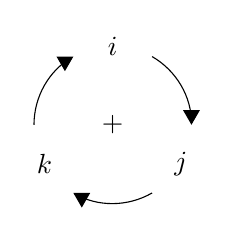
\begin{tikzpicture}[x=10mm, y=10mm]
%	\draw (0,0) circle (1.3);
	\coordinate (I) at (0,1);
	\coordinate (J) at ({cos(-30)},{sin(-30)});
	\coordinate (K) at ({cos(210)},{sin(210)});
	\draw (I) node {$i$};
	\draw (J) node {$j$};
	\draw (K) node {$k$};
	\draw [triangle 60-] (1,0) arc (0:60:1);
	\draw [triangle 60-] ({cos(120)},{sin(120)}) arc (120:180:1);
	\draw [triangle 60-] ({cos(240)},{sin(240)}) arc (240:300:1);
	\draw (0,0) node {$+$};

\end{tikzpicture}
\hfil
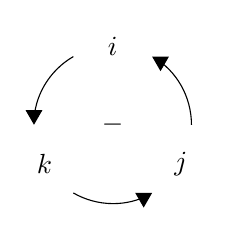
\begin{tikzpicture}[x=10mm, y=10mm]
%	\draw (0,0) circle (1.3);
	\coordinate (I) at (0,1);
	\coordinate (J) at ({cos(-30)},{sin(-30)});
	\coordinate (K) at ({cos(210)},{sin(210)});
	\draw (I) node {$i$};
	\draw (J) node {$j$};
	\draw (K) node {$k$};
	\draw [-triangle 60] (1,0) arc (0:60:1);
	\draw [-triangle 60] ({cos(120)},{sin(120)}) arc (120:180:1);
	\draw [-triangle 60] ({cos(240)},{sin(240)}) arc (240:300:1);
	\draw (0,0) node {$-$};

\end{tikzpicture}
\hfil

\

The inverse of a quaternion is given by:

$$ (a + bi + cj + dk)^{-1} = \frac{a - bi - cj - dk}{a^2 + b^2 + c^2 + d^2}$$

\

{\bf Vector Form of Quaternions}

Think of $a + bi + cj + dk$ as the pair, $(a, \langle b,c,d \rangle )$, with a scalar part and a vector part.  

Then quaternion addition is \ $(r_1, \vec{v}_1) + (r_2, \vec{v}_2) = (r_1 + r_2, \vec{v}_1 + \vec{v}_2)$.

Vector multiplication is $(r_1,\vec{v}_1) (r_2,\vec{v}_2) = (r_1r_2 - \vec{v}_1 \cdot \vec{v}_2, \ r_1\vec{v}_2 + r_2 \vec{v}_1 + \vec{v}_1 \times \vec{v}_2)$


\subsection{Quaternions as Rotations}

We start with a vector, $\vec{p} = (p_x, p_y, p_z)$, written as a quaternion with real coordinate zero, 
$$p = p_x \mathbf{i} + p_y \mathbf{j} + p_z \mathbf{k}$$

We want a rotation of $p$ through an angle of $\theta$ about the axis defined by a unit vector $$\vec{u} =  ( u_x, u_y, u_z ) = u_x \mathbf{i} + u_y \mathbf{j} + u_z \mathbf{k}$$ 

In two dimensions, Euler's Formula,  $e^{i\theta} = \cos \theta + i \sin \theta$, gives a counterclockwise rotation of $\theta$.  We can extend it to three dimensions as
$$q = e^{ 
	\frac{\theta}{2}
	( u_x \mathbf{i} + u_y \mathbf{j} + u_z \mathbf{k} )
	}
=
	\cos \frac{\theta}{2} + ( u_x \mathbf{i} + u_y \mathbf{j} + u_z \mathbf{k} ) \sin \frac{\theta}{2}
$$

The rotation of $\vec{p}$ about $\vec{u}$ is given by 
$$p' = q p q^{-1}$$

Going back to using Euler's Formula for a rotation, let's look at the multiplicative inverse of $q$ and see that it's consistent with previous knowledge.  By a previous formula, 
$$a^{-1} = (a_w + a_x \mathbf{i} + a_y \mathbf{j} + a_z \mathbf{k})^{-1} = 
\frac{1}{a_w^2 + a_x^2 + a_y^2 + a_z^2} (a_w - a_x \mathbf{i} - a_y \mathbf{j} - a_z \mathbf{k} )$$

The vector $\vec{u} = u_x \mathbf{i} + u_y \mathbf{j} + u_z \mathbf{k}$ is a unit vector with real part zero, so the denominator is 1.  
$$(\vec{u})^{-1} = (u_x \mathbf{i} + u_y \mathbf{j} + u_z \mathbf{k})^{-1} = -u_x \mathbf{i} - u_y \mathbf{j} - u_z \mathbf{k} = -\vec{u}$$

Applying the extension of Euler's Formula, 
$$q = e^{ 
	\frac{\theta}{2}
	( u_x \mathbf{i} + u_y \mathbf{j} + u_z \mathbf{k} )
	}
=
	\cos \frac{\theta}{2} + ( u_x \mathbf{i} + u_y \mathbf{j} + u_z \mathbf{k} ) \sin \frac{\theta}{2}
$$

and the inverse formula

$$a^{-1} = (a_w + a_x \mathbf{i} + a_y \mathbf{j} + a_z \mathbf{k})^{-1} = 
\frac{1}{a_w^2 + a_x^2 + a_y^2 + a_z^2} (a_w - a_x \mathbf{i} - a_y \mathbf{j} - a_z \mathbf{k} )$$

we get

$$q^{-1} = \frac{1}{
	\cos^2 \frac{\theta}{2}
	 + u_x^2 \sin ^2 \frac{\theta}{2}
	 + u_y^2 \sin ^2 \frac{\theta}{2}
	 + u_z^2 \sin ^2 \frac{\theta}{2}
	}
	\left(\cos \frac{\theta}{2} - ( u_x \mathbf{i} + u_y \mathbf{j} + u_z \mathbf{k} ) \sin \frac{\theta}{2}\right)
$$

$$ = \frac{1}{
	\cos^2 \frac{\theta}{2}
	 + (u_x^2 
	 + u_y^2 
	 + u_z^2) \sin ^2 \frac{\theta}{2}
	}
	\left(\cos \left( - \frac{\theta}{2} \right) + ( u_x \mathbf{i} + u_y \mathbf{j} + u_z \mathbf{k} ) \sin \left(-\frac{\theta}{2}\right)\right)
$$

$$ = \frac{1}{
	\cos^2 \frac{\theta}{2}
	+ \sin ^2 \frac{\theta}{2}
	}
	\left(\cos \left( - \frac{\theta}{2} \right) + ( u_x \mathbf{i} + u_y \mathbf{j} + u_z \mathbf{k} ) \sin \left(-\frac{\theta}{2}\right)\right)
$$

$$ = e^{\frac{\theta}{2}(-u)} = \left(e^{\frac{\theta}{2}u}\right)^{-1}
$$


%%%%%%%%%%%%%%%%
\section{Thursday 23 August:  Raster Display v/s Vector Display}
%%%%%%%%%%%%%%%%%

\

{\bf Ray Tracing}:  Which objects intersect the line?

\

{\bf Polygon Projection (Polygon Rendering)}

Triangles on the screen

Vertex coordinates

Multiply by matrices to convert to screen's coordinate system

\

Modeling Coordinates 

\qquad $\to$ World Coordinates

\qquad $\to$ Viewing and Projection Coordinates (Camera View)

\qquad $\to$ Normalized Coordinates

\qquad $\to$ Device Coordinates

\

\begin{tabular}{m{0.3in}m{.2in}*4{m{1.0in}m{.2in}}}
	$\left[ \begin{matrix} x \cr y \cr z \cr w \cr \end{matrix}\right]$
	&
	$\to$
	&
	Model \par Martrix
	&
	$\to$
	&
	Projection \par Matrix \par (Camera View)
	&
	$\to$
	&
	Perspective \par Division
	&
	$\to$
	&
	Viewpoint \par Transformation
	\cr
\end{tabular}

\

{\bf 2D Scan Conversion}:  Converts 2D object description to pixel values. 

{\it ``Pixel''}  Picture Element

Visible Surface Determination:  Occlusion

\

Direct Illumination v/s Global Illumination:  Shadows not completely dark

Curves and surfaces give a smooth alternative to polygonal representation of objects.  

\

Lots of student projects have dealt with {\bf Particle Dynamics}

\

{\bf Early Video Games}  Nimatron (1940) had columns of lights.   First ``video'' game, ``CRT Amusement Device,'' used an oscilloscope as its screen.  

\

{\bf Raster Display} - Image broken into pixels

{\bf Vector Display} - Smooth curves, like moving lasers or electron beam.  

\

Black \& white {\bf bitmap} has one bit per pixel

\

{\bf Raster Displays}

More computationally expensive

Requires more memory

Constant refresh rate

Supports area fills

Won over vector after memory got cheap.  

\

Frame buffers are getting more complex.  

\qquad Double buffering so screen doesn't refresh in the middle of a memory move

\qquad Left and right buffers for stereoscopic rendering

\qquad Depth buffer for occlusion

\

{\bf Know from Today's Lesson}

Pixel, raster, bitmap, frame buffer, {\it aliasing}

Know the difference between raster and vector.  

\

{\bf Aliasing} - in computer graphics, the jagged, or saw-toothed appearance of curved or diagonal lines on a low-resolution monitor.


%%%%%%%%%%%%%%
\section{Tuesday 28 August:  Scan Conversion of a Line Segment}
%%%%%%%%%%%%%%%%

{\bf Simplifying Assumptions}

1-pixel-thick line on a B\&W display (monochrome)

$m \in [-1,1]$.  More elaborate code can deal with other slopes.

Line segment described by two integer endpoints (endpoints fall exactly on pixels) $(x_s,y_s), (x_e,y_e)$

\

\hfil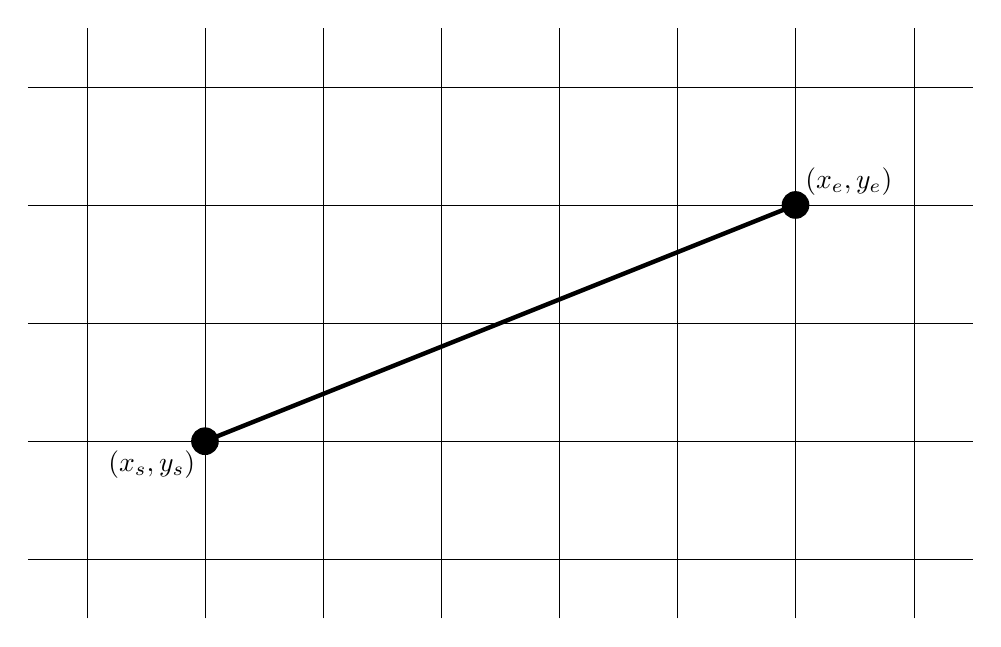
\begin{tikzpicture}[x=15mm, y=15mm]
	\foreach \i in {0,1,2,...,4}{
		\draw [ultra thin] (-0.5,\i) -- (7.5,\i);
	}
	\foreach \i in {0,1,2,...,7}{
		\draw [ultra thin] (\i,-0.5) -- (\i,4.5);
	}
	\coordinate (S) at (1,1);
	\coordinate (E) at (6,3);
	\fill (S) circle (5pt) node [below left] {$(x_s,y_s)$};
	\fill (E) circle (5pt) node [above right] {$(x_e,y_e)$};
	\draw [ultra thick] (S) -- (E);
\end{tikzpicture}

{\bf Main Idea}:  Activate one pixel per column from $x_s$ to $x_e$.  

\

\hfil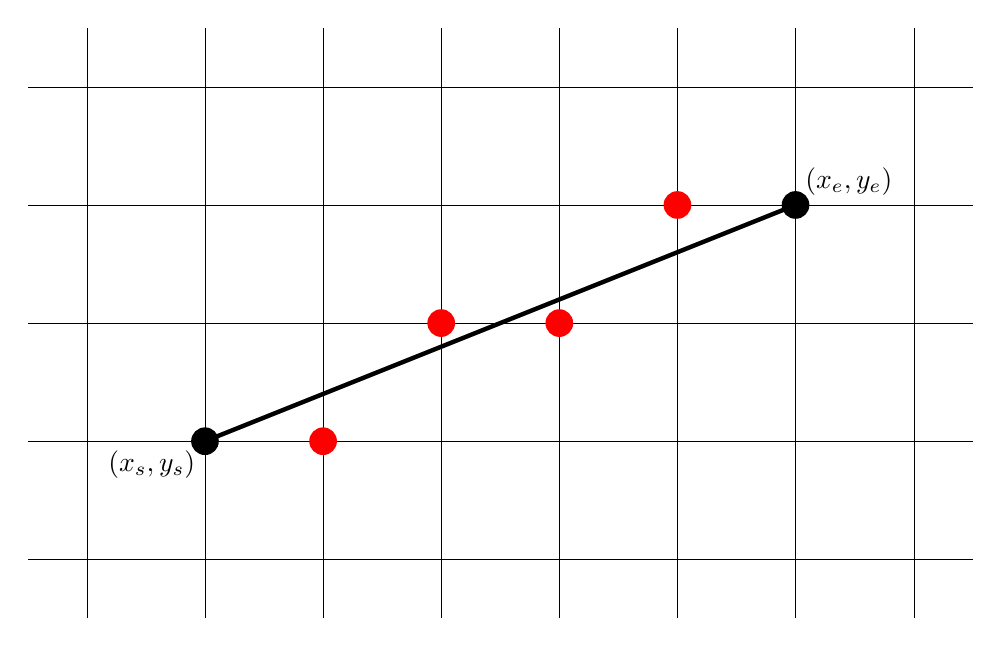
\begin{tikzpicture}[x=15mm, y=15mm]
	\foreach \i in {0,1,2,...,4}{
		\draw [ultra thin] (-0.5,\i) -- (7.5,\i);
	}
	\foreach \i in {0,1,2,...,7}{
		\draw [ultra thin] (\i,-0.5) -- (\i,4.5);
	}
	\coordinate (S) at (1,1);
	\coordinate (E) at (6,3);
	\fill (S) circle (5pt) node [below left] {$(x_s,y_s)$};
	\fill (E) circle (5pt) node [above right] {$(x_e,y_e)$};
	\draw [ultra thick] (S) -- (E);
	\fill [red] (2,1) circle (5pt);
	\fill [red] (3,2) circle (5pt);
	\fill [red] (4,2) circle (5pt);
	\fill [red] (5,3) circle (5pt);
\end{tikzpicture}

{\bf Simple, but Slow, Algorithm}

$m = (y_e - y_s) / (x_e - x_s)$

$b = y_s - m \cdot x_s$

for $x$ from $x_s$ to $x_e$ {\color{red} \it (inclusive)}

\qquad color pixel at $(x, \lfloor m \cdot x + b + 0.5 \rfloor)$

\

The problem with this algorithm that is the $m \cdot x$, floating-point multiplication, is really computationally expensive, usually six cycles, while addition is relatively cheap, usually one cycle.  

\

Rendering algorithms have to be as fast as possible, because they run billions of times.  

\

{\bf Basic Incremental Algorithm (DDA, Digital Differential Analyzer)}

$m = (y_e - y_s) / (x_e - x_s)$

$b = y_s - m \cdot x_s$

$x_0 = x_s$

$y_0 = y_s$

for $i$ from 1 to $(x_e - x_s)$

\qquad $(x_{i+1}, y_{i+1}) = (x_i + 1, y_i + m)$

\qquad color pixel at $(x_i+1, \lfloor y_{i+1} + 0.5 \rfloor )$ 

\

{\bf Midpoint Algorithm (Besenham)}

Developed for pen plotter.

Bottleneck was algorithm and computational speed, not hardware speed.

\

Simplifying assumption:  $m \in [0,1]$

\

Main idea

\qquad Move either E or NE in each move.  

\qquad Choose based on value of decision variable, $d$, which lets us choose betwen E and NE.  

\

\

\hfil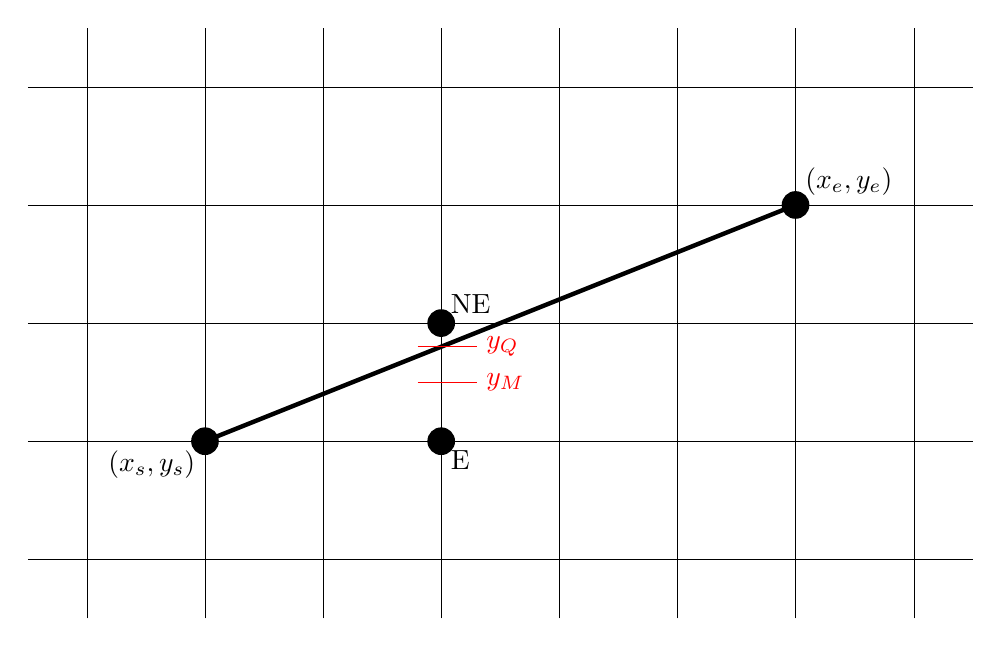
\begin{tikzpicture}[x=15mm, y=15mm]
	\foreach \i in {0,1,2,...,4}{
		\draw [ultra thin] (-0.5,\i) -- (7.5,\i);
	}
	\foreach \i in {0,1,2,...,7}{
		\draw [ultra thin] (\i,-0.5) -- (\i,4.5);
	}
	\coordinate (S) at (1,1);
	\coordinate (E) at (6,3);
	\fill (S) circle (5pt) node [below left] {$(x_s,y_s)$};
	\fill (E) circle (5pt) node [above right] {$(x_e,y_e)$};
	\draw [ultra thick] (S) -- (E);
	\draw [red] (2.8,1.8) -- (3.3,1.8) node [right, red] {$y_Q$};
	\draw [red] (2.8,1.5) -- (3.3,1.5) node [right, red] {$y_M$};
	\fill (3,1) circle (5pt) node [below right] {E};
	\fill (3,2) circle (5pt) node [above right] {NE};
\end{tikzpicture}

Notation:   $Q$ for {\it crossing}, $M$ for {\it midpoint}.

\

{\bf Algorithm}

$d = y_Q - y_M$.  

Look at sign of $d$.  

Move NE when $d$ is positive.

Move E otherwise.  

\

{\bf Computing $d$}

Initialize $d = m - 0.5$

Increment:

\qquad for E moves:  $d = d+m$

\qquad for NE moves:  $d = d + m - 1$

\

Here's how Midpoint is cheaper than DDA:  We can change everything to integers and not have any floats.  

\

{\bf Make Everything Integers}

Scale everything by $2 \Delta x$, so that $m - 0.5$ becomes an integer.  

$d = 2 \Delta y - \Delta x$

East increment:  $d = d + 2 \Delta y$

NE increment:  $d = d + 2 \Delta y - 2 \Delta x$

\

These methods aren't what we use today.  Probably triangle scan conversion.  


%%%%%%%%%
\section{Thursday 30 August:  Scan Conversion of a Triangle}
%%%%%%%%%%%

\subsection{Homework 1} due 13 September

{\it Callback}  Do sth when sth happens

Will have global variables

Assignment is given as a triangle with a certain order of $x_0$, $x_1$, and $x_2$.  Extra part of assignment is to account for different orders.  

\

\subsection{Midpoint Algorithm (Besenham) Pseudocode}

Initialize integers $\Delta_E$, $\Delta_{NE}$, $d$, $x$, and $y$.  

Set pixel at $(x,y)$ (first pixel)

\

{\bf while} $x$ $<$ last column (given by an endpoint)

\{

	\qquad increment $x$ by 1
	
	\qquad {\bf if} ($d<0$)
	
		\qquad \qquad add $\Delta _E$ to $d$
	
	\qquad {\bf else}
	
	\qquad \{
	
		\qquad \qquad increment $y$ by 1
		
		\qquad \qquad add $\Delta_{NE}$ to $d$
	
	\qquad \}
	
	\qquad set pixel at $(x,y)$

\}

\

\subsection{Naming Conventions}

\hfil\begin{tikzpicture}[x=16mm, y=16mm]
	\coordinate (A) at (0,0);
	\coordinate (B) at (-4,4);
	\coordinate (C) at (2,6);
	\draw (A) -- (B) -- (C) -- (A);
	\path (A) node [below] {$(x_0,y_0,R_0,G_0,B_0)$};
	\path (B) node [left] {$(x_1,y_1,R_1,G_1,B_1)$};
	\path (C) node [above] {$(x_2,y_2,R_2,G_2,B_2)$};
	
	\coordinate (M01) at (-2,2);
	\coordinate (L01) at ($(M01) - ({1/sqrt(2)},{1/sqrt(2)})$);
	\node (NM01) at (M01) {};
	\node (NL01) at (L01) {$L_{0,1}$};
	\draw [->] (NL01) -- (NM01);

	\coordinate (M02) at (1,3);
	\coordinate (L02) at ($(M02) + ({3/sqrt(10)},{-1/sqrt(10)})$);
	\node (NM02) at (M02) {};
	\node (NL02) at (L02) {$L_{0,2}$};
	\draw [->] (NL02) -- (NM02);

	\coordinate (M12) at (-1,5);
	\coordinate (L12) at ($(M12) + ({-1/sqrt(10)},{3/sqrt(10)})$);
	\node (NM12) at (M12) {};
	\node (NL12) at (L12) {$L_{1,2}$};
	\draw [->] (NL12) -- (NM12);

\end{tikzpicture}

Simplifying Assumptions:

\qquad Vertices have integer coordinates

\qquad $y_0 \le y_1 \le y_2$

\

{\bf Idea}

We want to interpolate the colors to get shading.  

Look at the triangle one scan line at a time, looping bottom to top, left to right.  

\

Two loops

\qquad One for the bottom

\qquad One for the top

\

\hfil\begin{tikzpicture}[x=8mm, y=8mm]
	\coordinate (V0) at (0,0);
	\coordinate (V1) at (-4,4);
	\coordinate (V2) at (2,6);
	\draw (V0) -- (V1) -- (V2) -- (V0);
	\path (V0) node [below] {$(x_0,y_0,R_0,G_0,B_0)$};
	\path (V1) node [left] {$(x_1,y_1,R_1,G_1,B_1)$};
	\path (V2) node [above] {$(x_2,y_2,R_2,G_2,B_2)$};
	
	\coordinate (M01) at ($(V0)!0.5!(V1)$);
	\coordinate (L01) at ($(M01) - ({1/sqrt(2)},{1/sqrt(2)})$);
	\node (NM01) at (M01) {};
	\node (NL01) at (L01) {$L_{0,1}$};
	\draw [->] (NL01) -- (NM01);

	\coordinate (M02) at ($(V0)!0.5!(V2)$);
	\coordinate (L02) at ($(M02) + ({3/sqrt(10)},{-1/sqrt(10)})$);
	\node (NM02) at (M02) {};
	\node (NL02) at (L02) {$L_{0,2}$};
	\draw [->] (NL02) -- (NM02);

	\coordinate (M12) at ($(V1)!0.5!(V2)$);
	\coordinate (L12) at ($(M12) + ({-1/sqrt(10)},{3/sqrt(10)})$);
	\node (NM12) at (M12) {};
	\node (NL12) at (L12) {$L_{1,2}$};
	\draw [->] (NL12) -- (NM12);
	
	\draw [dashed] (V1) -- ({4/3},4);
	
\end{tikzpicture}

\

{\bf Scan Line}

\

\hfil\begin{tikzpicture}[x=16mm, y=16mm]
	\coordinate (V0) at (0,0);
	\coordinate (V1) at (-4,4);
	\coordinate (V2) at (2,6);
	\draw (V0) -- (V1) -- (V2) -- (V0);
	\path (V0) node [below] {$(x_0,y_0,R_0,G_0,B_0)$};
	\path (V1) node [left] {$(x_1,y_1,R_1,G_1,B_1)$};
	\path (V2) node [above] {$(x_2,y_2,R_2,G_2,B_2)$};
	
	\coordinate (M01) at ($(V0)!0.8!(V1)$);
	\coordinate (L01) at ($(M01) - ({1/sqrt(2)},{1/sqrt(2)})$);
	\node (NM01) at (M01) {};
	\node (NL01) at (L01) {$L_{0,1}$};
	\draw [->] (NL01) -- (NM01);

	\coordinate (M02) at ($(V0)!0.8!(V2)$);
	\coordinate (L02) at ($(M02) + ({3/sqrt(10)},{-1/sqrt(10)})$);
	\node (NM02) at (M02) {};
	\node (NL02) at (L02) {$L_{0,2}$};
	\draw [->] (NL02) -- (NM02);

	\coordinate (M12) at ($(V1)!0.5!(V2)$);
	\coordinate (L12) at ($(M12) + ({-1/sqrt(10)},{3/sqrt(10)})$);
	\node (NM12) at (M12) {};
	\node (NL12) at (L12) {$L_{1,2}$};
	\draw [->] (NL12) -- (NM12);
	
	\draw [dashed] (V1) -- ({4/3},4);
	
	\coordinate (sL) at (-3,1.5);
	\coordinate (sR) at (2,1.5);
	\draw [dashed] (sL) -- (sR) node [right] {Scan line};
	
	\coordinate (xL) at (intersection of V0--V1 and sL--sR);
	\coordinate (xR) at (intersection of V0--V2 and sL--sR);
	\fill (xL) circle (5pt) node [below left] {$(x_L,y)$};
	\fill (xR) circle (5pt) node [below right] {$(x_R,y)$};

\end{tikzpicture}

\subsection{Line Scan Pseudocode}

for $y$ from $y_0$ to $(y_1 - 1)$

\{

\qquad Calculate coordinates where scan line intersects $L_{0,1}$ and $L_{0,2}$.  

\qquad \qquad ({\it i.e.} Calculate $x_L$ and $x_R$ incrementally)

\qquad Color the pixels from $\left( \lceil x_L \rceil, y \right)$ to $\left( \lfloor x_R \rfloor, y \right)$


\}



\

for $y$ from $y_1$ to $y_2$

\{

\qquad Calculate coordinates where scan line intersects $L_{1,2}$ and $L_{0,2}$.  

\qquad \qquad ({\it i.e.} Calculate $x_L$ and $x_R$ incrementally)

\qquad Color the pixels from $\left( \lceil x_L \rceil, y \right)$ to $\left( \lfloor x_R \rfloor, y \right)$


\}

\subsection{Special Cases}

{\bf Watch for division by zero!}

Horizontal lines, either between $V_0$ and $V_1$ or between $V_1$ and $V_2$.  

\subsection{Calculating $x_L$ and $x_R$ Incrementally}

\begin{tabular}{p{4in}p{2in}}

Initialize $x_L = x_0$, $x_R = x_0$, $y = y_0$

Note that $y$ is being incremented by 1.  
\

$\displaystyle x_{i+1} = x_i + \frac{1}{m} = x_i + \frac{x_1 - x_0}{y_1 - y_0}$

\

$\displaystyle x_L = x_L +  + \frac{x_1 - x_0}{y_1 - y_0}$

\

$\displaystyle x_R = x_R +  + \frac{x_2 - x_0}{y_2 - y_0}$

&
\hfill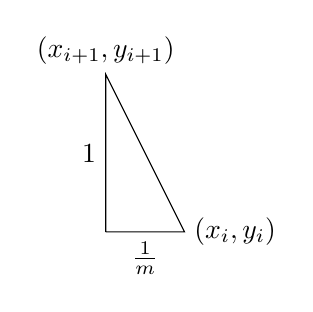
\begin{tikzpicture}[baseline=(current bounding box.north),x=10mm, y=10mm]
	\coordinate (A) at (0,0);
	\coordinate (B) at (1,0);
	\coordinate (C) at (0,2);
	\draw (A) -- (B) -- (C) -- (A);
	\path (B) node [right] {$(x_i,y_i)$};
	\path (C) node [above] {$(x_{i+1}, y_{i+1})$};
	\path (A) -- (B) node [midway, below] {$\frac{1}{m}$};
	\path (A) -- (C) node [midway, left] {1};
\end{tikzpicture}

\cr
\end{tabular}

\subsection{Color}

{\color{red}
	Notes on this section:  
	
	Make sure we're consistent about when to use $x_L - x_R$ and when to use $\lceil x_L \rceil - \lfloor x_R \rfloor$.
}

\

Computing color incrementally (Here considering only R, red)

Initialize $R_L = R_0$, $R_R = R_0$

For each scan line:

\

\qquad $\displaystyle R_L = R_L + \frac{R_1 - R_0}{y_1 - y_0}$

\

\qquad $\displaystyle R_R = R_R + \frac{R_2 - R_0}{y_2 - y_0}$

\

Within a scan line, between $\lceil x_L \rceil$ and $\lfloor  x_R \rfloor$

\

\qquad Initialize $\displaystyle R = R_L + \frac{R_L - R_R}{x_L - x_R} \left( \lceil x_L \rceil - x_L \right)$

\qquad Color first pixel

\qquad for $R$ from $R_L$ to $R_R$

\qquad \{

\qquad \qquad $\displaystyle R = R + \frac{R_L - R_R}{\lceil x_L \rceil - \lfloor x_R \rfloor } $

\qquad \qquad [Do the same for $G$ and $B$.]

\qquad \qquad Color pixel $(x, y, R, G, B)$

\qquad \}


%%%%%%%%%%%%
\section{Running OpenGL on a Mac}
%%%%%%%%%%%%%

\subsection{Installing OpenGL}

You don't have to.  It comes in the box.  

\subsection{Visual Studio}

\url{https://social.msdn.microsoft.com/Forums/en-US/ef99e9f5-2a48-423b-b6c0-fa5617d7c63d/how-do-i-get-c-to-work-on-visual-studio-for-mac?forum=visualstudiogeneral}

This post was from March 2017, but I think it's still true.  The Microsoft person says that Visual Studio for Mac is designed for building mobile apps, not for general computing.  It does not support {\tt C++}.  She kindly recommends that you run Windows.  

\subsection{How Brad Does It}

\begin{itemize}
	\item Install GLEW and GLFW.  The easiest way to do it is with Homebrew, which is one of the programs you can install that lets you unleash the Linux power of your Mac.  
	
	{\tt brew install glew}
	
	Another way to do it is to download the .zip files from the GLEW and GLFW websites and build.  GLEW comes with a {\tt Makefile}, but for GLFW you have to use CMake.  
	
	\item Link your code to {\tt glew.h} and {\tt glfw3.h}.  
	
	One way to link your code to the library is to replace the 
	\begin{verbatim}#include <GLFW/glfw3.h>\end{verbatim}
	with the path to the {\tt glfw3} file on your machine, something like 
	\begin{verbatim}#include </usr/local/Cellar/glfw/3.2.1/include/GLFW/glfw3.h>\end{verbatim}
	
	\item Tell OpenGL which version you want to use.  
	
	If you want to run an earlier version of OpenGL, as in Assignment 1 (so you can use {\tt glDrawPixels}, which was removed from the language in Version 3.2), ignore this step, and it will default to 2.1.
	
	This trick only works on my Mac if I specify version 3.3.   
	
	Put this code in your {\tt main()} function.
	
\begin{verbatim}	
      glfwWindowHint(GLFW_CONTEXT_VERSION_MAJOR, 3);
      glfwWindowHint(GLFW_CONTEXT_VERSION_MINOR, 3);
      glfwWindowHint(GLFW_OPENGL_FORWARD_COMPAT, GL_TRUE);
      glfwWindowHint(GLFW_OPENGL_PROFILE, GLFW_OPENGL_CORE_PROFILE);	
 \end{verbatim}
 
 \item Compile and Link.  
 
 I use {\tt g++}, the GNU compiler for {\tt C++}.  I use it not just because I'm old (which I am), but because I often run my big jobs in parallel on remote UNIX clusters, and they don't have integrated development environments (IDE's) like Visual Studio.  You have to do everything from a UNIX command line.  Since I have to be proficient in those tools anyway, I use them on my local computer.  
 
 Here's the command I use to compile and link my code.  
 
 {\tt g++ Assignment1.cpp -framework OpenGL -lGLEW -lGLFW}
 
\end{itemize}

\subsection{How Other People Do It}
 
 Send me your stories and I'll put them in.  
 

 %%%%%%%%%%%%%%%%
 \section{Tuesday 4 September:  Clipping}
 %%%%%%%%%%%%%%%%%%%%%
 
 \subsection{Cohen-Sutherland Line Clipper}
 
 We don't want to scan-convert things outside the viewing window.  Throw away the part of the line outside the window.  
 
 {\it Culling} is different.  That's throwing out objects that do not intersect the window at all.

\

\begin{tabular}{m{50mm}m{100mm}} 
 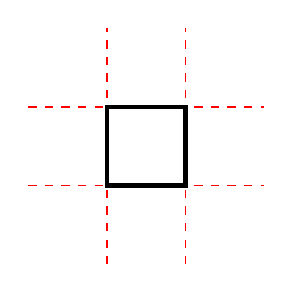
\begin{tikzpicture}[x=5mm, y=5mm]
 	\draw [red, dashed] (-3,1) -- (3,1);
	\draw [red, dashed] (-3,-1) -- (3,-1);
	\draw [red, dashed] (-1,-3) -- (-1,3);
	\draw [red, dashed] (1,-3) -- (1,3);
	\draw [ultra thick] (1,1) rectangle (-1,-1);
 \end{tikzpicture}
 &
 Each of these red dashed lines divides the plane into ``inner'' and ``outer'' sections.

\end{tabular}
 
\begin{tabular}{m{90mm}m{60mm}} 
 \begin{tikzpicture}[x=15mm, y=15mm]
 	\draw [red, dashed] (-3,1) -- (3,1);
	\draw [red, dashed] (-3,-1) -- (3,-1);
	\draw [red, dashed] (-1,-3) -- (-1,3);
	\draw [red, dashed] (1,-3) -- (1,3);
	\draw [ultra thick] (1,1) rectangle (-1,-1);
	\path (0,0) node {\tt 0000};
	\path (-2,2) node {\tt 1001};
	\path (0,2) node {\tt 1000};
	\path (2,2) node {\tt 1010};
	\path (-2,0) node {\tt 0001};
	\path (2,0) node {\tt 0010};
	\path (-2,-2) node {\tt 0101};
	\path (0,-2) node {\tt 0100};
	\path (2,-2) node {\tt 0110};
 \end{tikzpicture}
 &
 {\bf Encoding}

{\it Region out-codes}

\
 
 Pick an order (and be consistent)
 
 \
 
Dr. Borst's order in today's class:  Top, Bottom, Right, Left

\

Encode each sector with a four-digit binary code in which each digit tells whether the points are inside (0) or outside (1) the boundary.

\

``On the line'' counts as inside.  

 \end{tabular}
 
\begin{tabular}{m{60mm}m{90mm}} 

{\bf Iterative Algorithm}

Assign codes to segment endpoints.

\

{\tt IF} the segment is entirely in the window (both codes {\tt 0000})

\qquad Accept the segment

\

{\tt ELIF} both endpoints are outside a common boundary, {\it e.g.} both to the left, {\it i.e.} logical {\tt AND} of codes is nonzero,

\qquad Reject the segment.

\qquad (Same as culling.)

\

{\tt ELSE}  

\qquad Cut segment at a boundary

\qquad Discard the outer part

\qquad Run C-S Clipper on the inner part.  

&
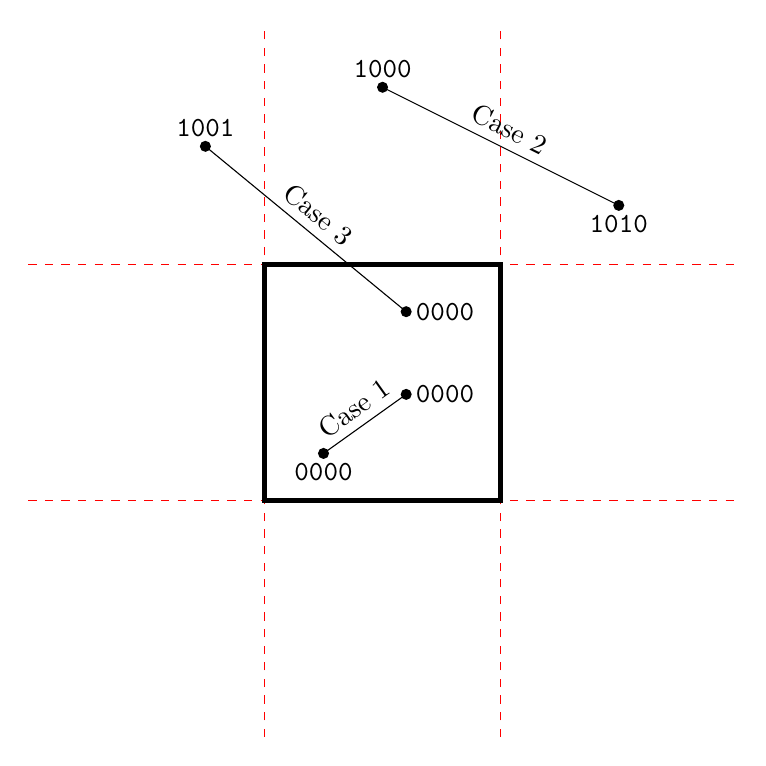
\begin{tikzpicture}[x=1.5mm, y=1.5mm]
 	\draw [red, dashed] (-30,10) -- (30,10);
	\draw [red, dashed] (-30,-10) -- (30,-10);
	\draw [red, dashed] (-10,-30) -- (-10,30);
	\draw [red, dashed] (10,-30) -- (10,30);
	\draw [ultra thick] (10,10) rectangle (-10,-10);

	\coordinate (A) at (-5,-6);
	\coordinate (B) at (2,-1);
	\fill (A) circle (2pt) node [below] {\tt 0000};
	\fill (B) circle (2pt) node [right] {\tt 0000};
	\draw (A) -- (B);
	\path (A) -- (B) node [midway, sloped, above] {Case 1};

	\coordinate (C) at (0,25);
	\coordinate (D) at (20,15);
	\fill (C) circle (2pt) node [above] {\tt 1000};
	\fill (D) circle (2pt) node [below] {\tt 1010};
	\draw (C) -- (D);
	\path (C) -- (D) node [midway, sloped, above] {Case 2};

	\coordinate (E) at (-15,20);
	\coordinate (F) at (2,6);
	\fill (E) circle (2pt) node [above] {\tt 1001};
	\fill (F) circle (2pt) node [right] {\tt 0000};
	\draw (E) -- (F) node [midway, sloped, above] {Case 3};

 \end{tikzpicture}
 \end{tabular}
 
{\bf To Cut the Line}

Pick an outside (not {\tt 0000}) endpoint.

Walk through the four digits left to right.

Identify the first nonzero bit in the code.

Cut the line at the boundary that corresponds to that bit.  

Lather, rinse, repeat.  

\

\begin{tabular}{@{}m{90mm}m{60mm}} 

1.  Scan the point codes left to right and pick the first one with a {\tt 1}.  There will be only one, because if they both had a {\tt 1} in the same position, they would have already been eliminated as being outside the same boundary.  Choose {\tt 1010}.

&
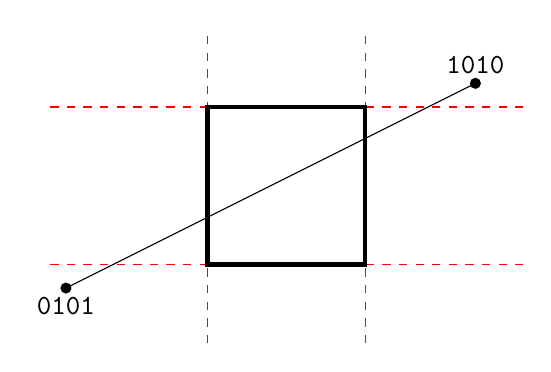
\begin{tikzpicture}[x=1.0mm, y=1.0mm]
 	\draw [red, dashed] (-30,10) -- (30,10);
	\draw [red, dashed] (-30,-10) -- (30,-10);
	\draw [red, dashed] (-10,-20) -- (-10,20);
	\draw [red, dashed] (10,-20) -- (10,20);
	\draw [ultra thick] (10,10) rectangle (-10,-10);

	\coordinate (A) at (-28,-13);
	\coordinate (B) at (24,13);
	\fill (A) circle (2pt) node [below] {\tt 0101};
	\fill (B) circle (2pt) node [above] {\tt 1010};
	\draw (A) -- (B);
	
	\coordinate (C) at (-22,-10);
	\coordinate (D) at (-10,-4);
	\coordinate (E) at (10,6);
	\coordinate (F) at (18,10);
	
%	\fill (C) circle (2pt) node [above left] {\tt 0001};
%	\fill (D) circle (2pt) node [above left] {\tt 0000};
%	\fill (E) circle (2pt) node [below right] {\tt 0000};
%	\fill (F) circle (2pt) node [below right] {\tt 0010};

 \end{tikzpicture}
 \end{tabular}
 
\

\begin{tabular}{@{}m{90mm}m{60mm}} 

2.  In {\tt 1010}, scan left to right to find the first {\tt 1}, which here represents ``Top."  Cut at the top boundary.  

\

3.  Check to see whether both points have encoding {\tt 0000}.  If they do, accept and end.   If not, check to see whether the encodings of the two points share a {\tt 1}.  If they do, reject the line.  

\

4.  Scan the point codes left to right and pick the first one with a {\tt 1}.  Choose {\tt 0101}.


&
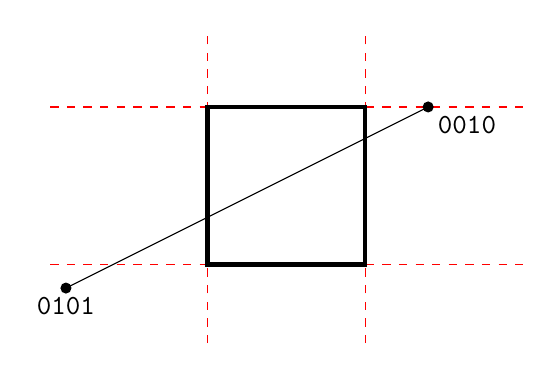
\begin{tikzpicture}[x=1.0mm, y=1.0mm]
 	\draw [red, dashed] (-30,10) -- (30,10);
	\draw [red, dashed] (-30,-10) -- (30,-10);
	\draw [red, dashed] (-10,-20) -- (-10,20);
	\draw [red, dashed] (10,-20) -- (10,20);
	\draw [ultra thick] (10,10) rectangle (-10,-10);

	\coordinate (A) at (-28,-13);
	\coordinate (B) at (24,13);
	\coordinate (C) at (-22,-10);
	\coordinate (D) at (-10,-4);
	\coordinate (E) at (10,6);
	\coordinate (F) at (18,10);
	
	\fill (A) circle (2pt) node [below] {\tt 0101};
%	\fill (C) circle (2pt) node [above left] {\tt 0001};
%	\fill (D) circle (2pt) node [above left] {\tt 0000};
%	\fill (E) circle (2pt) node [below right] {\tt 0000};
	\fill (F) circle (2pt) node [below right] {\tt 0010};
%	\fill (B) circle (2pt) node [above] {\tt 1010};

	\draw (A) -- (F);
	

 \end{tikzpicture}
 \end{tabular}
 
\

\begin{tabular}{@{}m{90mm}m{60mm}} 

5.  In {\tt 0101}, scan left to right to find the first {\tt 1}, which here represents ``Bottom."  Cut at the bottom boundary.  

\

6.  Check to see whether both points have encoding {\tt 0000}.  If they do, accept and end.  If not, check to see whether the encodings of the two points share a {\tt 1}.  If they do, reject the line.  

\

7.  Scan the point codes left to right and pick the first one with a {\tt 1}.  Choose {\tt 0010}.


&
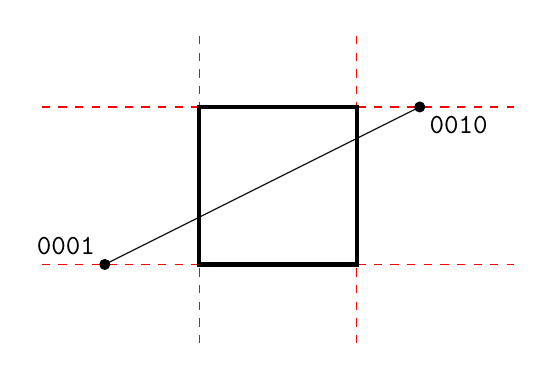
\begin{tikzpicture}[x=1.0mm, y=1.0mm]
 	\draw [red, dashed] (-30,10) -- (30,10);
	\draw [red, dashed] (-30,-10) -- (30,-10);
	\draw [red, dashed] (-10,-20) -- (-10,20);
	\draw [red, dashed] (10,-20) -- (10,20);
	\draw [ultra thick] (10,10) rectangle (-10,-10);

	\coordinate (A) at (-28,-13);
	\coordinate (B) at (24,13);
	\coordinate (C) at (-22,-10);
	\coordinate (D) at (-10,-4);
	\coordinate (E) at (10,6);
	\coordinate (F) at (18,10);
	
%	\fill (A) circle (2pt) node [below] {\tt 0101};
	\fill (C) circle (2pt) node [above left] {\tt 0001};
%	\fill (D) circle (2pt) node [above left] {\tt 0000};
%	\fill (E) circle (2pt) node [below right] {\tt 0000};
	\fill (F) circle (2pt) node [below right] {\tt 0010};
%	\fill (B) circle (2pt) node [above] {\tt 1010};

	\draw (C) -- (F);
	

 \end{tikzpicture}
 \end{tabular}
 
\

\begin{tabular}{@{}m{90mm}m{60mm}} 

8.  In {\tt 0010}, scan left to right to find the first {\tt 1}, which here represents ``Right."  Cut at the right boundary.  

\

9.  Check to see whether both points have encoding {\tt 0000}.  If they do, accept and end.  If not, check to see whether the encodings of the two points share a {\tt 1}.  If they do, reject the line.  

\

10.  Scan the point codes left to right and pick the first one with a {\tt 1}.  Choose {\tt 0001}.


&
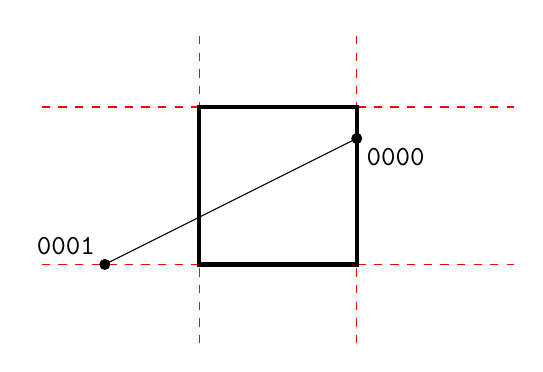
\begin{tikzpicture}[x=1.0mm, y=1.0mm]
 	\draw [red, dashed] (-30,10) -- (30,10);
	\draw [red, dashed] (-30,-10) -- (30,-10);
	\draw [red, dashed] (-10,-20) -- (-10,20);
	\draw [red, dashed] (10,-20) -- (10,20);
	\draw [ultra thick] (10,10) rectangle (-10,-10);

	\coordinate (A) at (-28,-13);
	\coordinate (B) at (24,13);
	\coordinate (C) at (-22,-10);
	\coordinate (D) at (-10,-4);
	\coordinate (E) at (10,6);
	\coordinate (F) at (18,10);
	
%	\fill (A) circle (2pt) node [below] {\tt 0101};
	\fill (C) circle (2pt) node [above left] {\tt 0001};
%	\fill (D) circle (2pt) node [above left] {\tt 0000};
	\fill (E) circle (2pt) node [below right] {\tt 0000};
%	\fill (F) circle (2pt) node [below right] {\tt 0010};
%	\fill (B) circle (2pt) node [above] {\tt 1010};

	\draw (C) -- (E);
	

 \end{tikzpicture}
 \end{tabular}
 
\

\

\begin{tabular}{@{}m{90mm}m{60mm}} 

11.  In {\tt 0001}, scan left to right to find the first {\tt 1}, which here represents ``Left."  Cut at the left boundary.  

\

12.  Check to see whether both points have encoding {\tt 0000}.  Since they do, accept and end.  

\



&
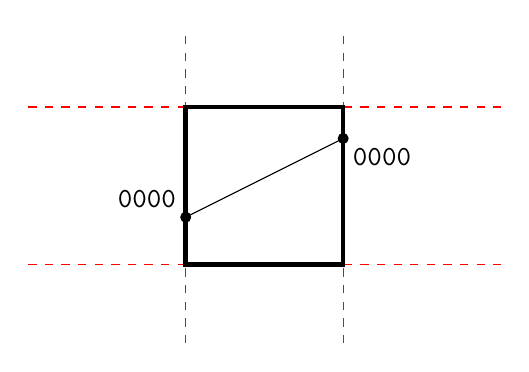
\begin{tikzpicture}[x=1.0mm, y=1.0mm]
 	\draw [red, dashed] (-30,10) -- (30,10);
	\draw [red, dashed] (-30,-10) -- (30,-10);
	\draw [red, dashed] (-10,-20) -- (-10,20);
	\draw [red, dashed] (10,-20) -- (10,20);
	\draw [ultra thick] (10,10) rectangle (-10,-10);

	\coordinate (A) at (-28,-13);
	\coordinate (B) at (24,13);
	\coordinate (C) at (-22,-10);
	\coordinate (D) at (-10,-4);
	\coordinate (E) at (10,6);
	\coordinate (F) at (18,10);
	
%	\fill (A) circle (2pt) node [below] {\tt 0101};
%	\fill (C) circle (2pt) node [above left] {\tt 0001};
	\fill (D) circle (2pt) node [above left] {\tt 0000};
	\fill (E) circle (2pt) node [below right] {\tt 0000};
%	\fill (F) circle (2pt) node [below right] {\tt 0010};
%	\fill (B) circle (2pt) node [above] {\tt 1010};

	\draw (D) -- (E);
	

 \end{tikzpicture}
 \end{tabular}
 
\

Generalizes to 3D.  

\subsection{Clipping Polygons}

{\color{red} Not clear about what to do with each vertex in the algorithm, whether to discard it or not.}

\

The math is a little more tedious, but not much.  

Window must be convex.

Convex casual definition:  If a bug walking around the perimeter only turns one way, it's convex.  

\

\begin{tabular}{m{75mm}m{85mm}}
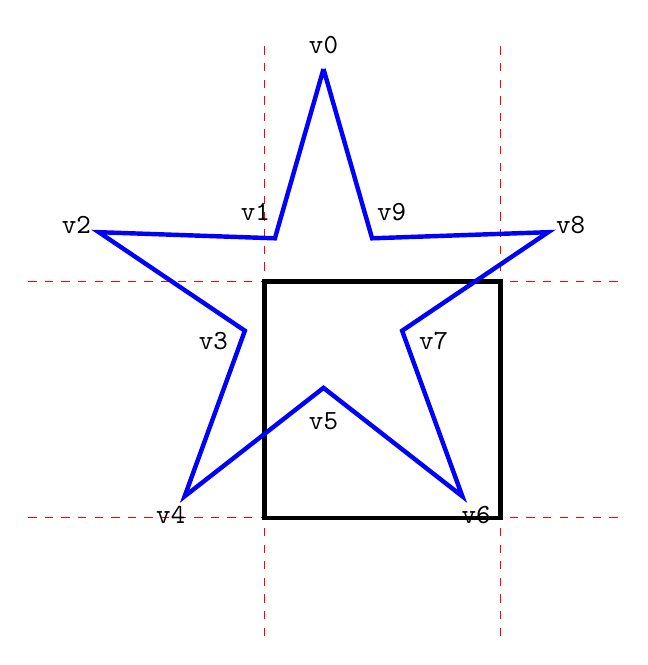
\begin{tikzpicture}[x=1.5mm,y=1.5mm]

	\coordinate (TL) at (-30,10);
	\coordinate (TR) at (20,10);
	\coordinate (BL) at (-30,-10);
	\coordinate (BR) at (20,-10);
	\coordinate (LB) at (-10,-20);
	\coordinate (LT) at (-10,30);
	\coordinate (RB) at (10,-20);
	\coordinate (RT) at (10,30);

 	\draw [red, dashed] (TL) -- (TR);
	\draw [red, dashed] (BL) -- (BR);
	\draw [red, dashed] (LB) -- (LT);
	\draw [red, dashed] (RB) -- (RT);
	\draw [ultra thick] (10,10) rectangle (-10,-10);
	
	\coordinate (v0) at ({-5+20*cos(90+0*36)},{8+20*sin(90+0*36)});
	\coordinate (v1) at ({-5+ 7*cos(90+1*36)},{8+ 7*sin(90+1*36)});
	\coordinate (v2) at ({-5+20*cos(90+2*36)},{8+20*sin(90+2*36)});
	\coordinate (v3) at ({-5+ 7*cos(90+3*36)},{8+ 7*sin(90+3*36)});
	\coordinate (v4) at ({-5+20*cos(90+4*36)},{8+20*sin(90+4*36)});
	\coordinate (v5) at ({-5+ 7*cos(90+5*36)},{8+ 7*sin(90+5*36)});
	\coordinate (v6) at ({-5+20*cos(90+6*36)},{8+20*sin(90+6*36)});
	\coordinate (v7) at ({-5+ 7*cos(90+7*36)},{8+ 7*sin(90+7*36)});
	\coordinate (v8) at ({-5+20*cos(90+8*36)},{8+20*sin(90+8*36)});
	\coordinate (v9) at ({-5+ 7*cos(90+9*36)},{8+ 7*sin(90+9*36)});
	
	\path ($1.1*(v0)-0.1*(-5,8)$) node {\tt v0};
	\path ($1.4*(v1)-0.4*(-5,8)$) node {\tt v1};
	\path ($1.1*(v2)-0.1*(-5,8)$) node {\tt v2};
	\path ($1.4*(v3)-0.4*(-5,8)$) node {\tt v3};
	\path ($1.1*(v4)-0.1*(-5,8)$) node {\tt v4};
	\path ($1.4*(v5)-0.4*(-5,8)$) node {\tt v5};
	\path ($1.1*(v6)-0.1*(-5,8)$) node {\tt v6};
	\path ($1.4*(v7)-0.4*(-5,8)$) node {\tt v7};
	\path ($1.1*(v8)-0.1*(-5,8)$) node {\tt v8};
	\path ($1.4*(v9)-0.4*(-5,8)$) node {\tt v9};
	
	\draw [blue, ultra thick] (v0) -- (v1) -- (v2) -- (v3) -- (v4) -- (v5) -- (v6) -- (v7) -- (v8) -- (v9) -- (v0);

\end{tikzpicture}
&
{\bf Algorithm}

Pick a boundary line.

Walk around in one direction, slicing the segments that intersect the boundary line.  

\

Top

{\tt v0 -- v1} is outside. Discard {\tt v0}.

{\tt v1 -- v2} is outside. Discard {\tt v1}.  

{\tt v2 -- v3} goes outside to inside. Make {\tt v10} at intersection.  Discard {\tt v2}.  

{\tt v3 -- v4} is inside.   Keep these vertices.  

$\vdots$

{\tt v7 -- v8} intersects.  Make {\tt v11} at intersection.  

\end{tabular}

New polygon is {\tt v10 -- v3 -- v4 -- v5 -- v6 -- v7 -- v11}

\begin{tabular}{m{100mm}m{60mm}}
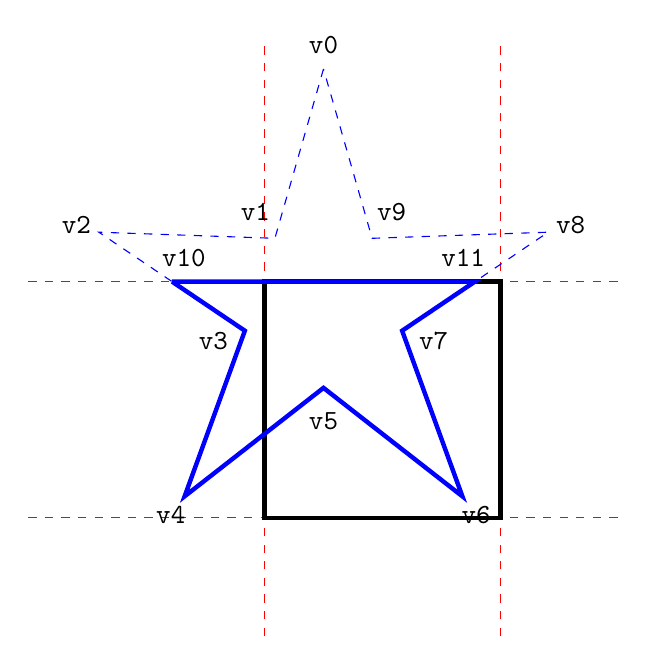
\begin{tikzpicture}[x=1.5mm,y=1.5mm]

	\coordinate (TL) at (-30,10);
	\coordinate (TR) at (20,10);
	\coordinate (BL) at (-30,-10);
	\coordinate (BR) at (20,-10);
	\coordinate (LB) at (-10,-20);
	\coordinate (LT) at (-10,30);
	\coordinate (RB) at (10,-20);
	\coordinate (RT) at (10,30);

 	\draw [red, dashed] (TL) -- (TR);
	\draw [red, dashed] (BL) -- (BR);
	\draw [red, dashed] (LB) -- (LT);
	\draw [red, dashed] (RB) -- (RT);
	\draw [ultra thick] (10,10) rectangle (-10,-10);
	
	\coordinate (v0) at ({-5+20*cos(90+0*36)},{8+20*sin(90+0*36)});
	\coordinate (v1) at ({-5+ 7*cos(90+1*36)},{8+ 7*sin(90+1*36)});
	\coordinate (v2) at ({-5+20*cos(90+2*36)},{8+20*sin(90+2*36)});
	\coordinate (v3) at ({-5+ 7*cos(90+3*36)},{8+ 7*sin(90+3*36)});
	\coordinate (v4) at ({-5+20*cos(90+4*36)},{8+20*sin(90+4*36)});
	\coordinate (v5) at ({-5+ 7*cos(90+5*36)},{8+ 7*sin(90+5*36)});
	\coordinate (v6) at ({-5+20*cos(90+6*36)},{8+20*sin(90+6*36)});
	\coordinate (v7) at ({-5+ 7*cos(90+7*36)},{8+ 7*sin(90+7*36)});
	\coordinate (v8) at ({-5+20*cos(90+8*36)},{8+20*sin(90+8*36)});
	\coordinate (v9) at ({-5+ 7*cos(90+9*36)},{8+ 7*sin(90+9*36)});
	
	\coordinate (v10) at (intersection of TL--TR and v2--v3);
	\coordinate (v11) at (intersection of TL--TR and v7--v8);

	
	\path ($1.1*(v0)-0.1*(-5,8)$) node {\tt v0};
	\path ($1.4*(v1)-0.4*(-5,8)$) node {\tt v1};
	\path ($1.1*(v2)-0.1*(-5,8)$) node {\tt v2};
	\path ($1.4*(v3)-0.4*(-5,8)$) node {\tt v3};
	\path ($1.1*(v4)-0.1*(-5,8)$) node {\tt v4};
	\path ($1.4*(v5)-0.4*(-5,8)$) node {\tt v5};
	\path ($1.1*(v6)-0.1*(-5,8)$) node {\tt v6};
	\path ($1.4*(v7)-0.4*(-5,8)$) node {\tt v7};
	\path ($1.1*(v8)-0.1*(-5,8)$) node {\tt v8};
	\path ($1.4*(v9)-0.4*(-5,8)$) node {\tt v9};
	
	\path ($(v10)+(1,2)$) node {\tt v10};
	\path ($(v11)+(-1,2)$) node {\tt v11};
	
	\draw [blue, dashed] (v0) -- (v1) -- (v2) -- (v3) -- (v4) -- (v5) -- (v6) -- (v7) -- (v8) -- (v9) -- (v0);
	\draw [blue, ultra thick] (v10) -- (v3) -- (v4) -- (v5) -- (v6) -- (v7) -- (v11) -- (v10);

\end{tikzpicture}
&

Repeat for other three boundary lines.  
\end{tabular}

\

Four cases moving from one vertex to the next.  

\begin{enumerate}
	\item Completely inside.  Add one vertex
	\item Crosses inside to outside.  Add one vertex.  
	\item Completely outside.  Do nothing.
	\item Cross outside to inside.  Add two vertices.  
\end{enumerate}


%%%%%%%%%%%
\section{Thursday 6 September:  Math Review}
%%%%%%%%%%%

Here I'm going to put things that Dr. Borst talked about that weren't in Jason's excellent talk, plus some thoughts that came to my mind.    

\

\subsection{Matrix Notation and Matrix-Matrix Multiplication (MMM)}

\

Let $\displaystyle
B = 
\left[
\begin{tabular}{rrr}
	1 & 2  \cr
	3 & 4 \cr
	5 & 6 \cr
\end{tabular}
\right]
$
and
$\displaystyle
C = \left[
\begin{tabular}{rrrr}
	7 & 8 & 9 & 10 \cr
	11 & 12 & 13 & 14 \cr
\end{tabular}
\right]
$

\

$B$ is a ``three by two'' matrix, and $C$ is a ``two by four''matrix.  The first number is the number of rows, and the second the columns.  

\

$B_{i,j}$ is the {\it element} of $B$ in the $i^{\text{th}}$ row and the $j^{\text{th}}$ column, so $B_{2,3} = 6$.  Note that we're counting the rows and columns starting at 1, not 0.  

\

To multiply the matrices, $A = B \times C$, we're using the dot product.  The value of $A_{i,j}$ is the dot product of row $i$ of $B$ and column $j$ of $C$.  Note that this multiplication can't happen if the number of columns of $B$ doesn't match the number of rows of $C$.  

\

$\displaystyle 
A_{2,3} = [3,4] \cdot
\left[ 
\begin{tabular}{rrr}
	9 \cr
	13 \cr
\end{tabular}
\right]
= 3 \cdot 9 + 4 \cdot 13 = 27 + 52 = 79
$

\
$\displaystyle
A = B \times C = 
\left[
\begin{tabular}{rrr}
	1 & 2  \cr
	3 & 4 \cr
	5 & 6 \cr
\end{tabular}
\right]
\cdot
\left[
\begin{tabular}{rrrr}
	7 & 8 & 9 & 10 \cr
	11 & 12 & 13 & 14 \cr
\end{tabular}
\right]
$

\

$\displaystyle = 
\left[
\begin{tabular}{*4{>{$}r<{$}}}
	1 \cdot 7 + 2 \cdot 11 & 
	1 \cdot 8 + 2 \cdot 12 &
	1 \cdot 9 + 2 \cdot 13 &
	1 \cdot 10 + 2 \cdot 14 \cr
	3 \cdot  7 + 4 \cdot 11 &
	3 \cdot  8 + 4 \cdot 12 &
	3 \cdot  9 + 4 \cdot 13 &
	3 \cdot  10 + 4 \cdot 14 \cr
	5 \cdot  7 + 6 \cdot 11  &
	5 \cdot  8 + 6 \cdot 12  &
	5 \cdot  9 + 6 \cdot 13  &
	5 \cdot  10 + 6 \cdot 14  \cr
\end{tabular}
\right]
=\left[
\begin{tabular}{*4{>{$}r<{$}}}
	29 & 32 & 35 & 38 \cr
	65 & 72 & 79 & 86 \cr
	101 & 112 & 123 & 134 \cr
\end{tabular}
\right]
$

\

In mathic notation, $\displaystyle A_{i,j} = \sum_{k=1}^2 B_{i,k} \times C_{k,j}$

\

In {\tt C++},

\

\begin{lstlisting}[language=C++, caption={Matrix-Matrix Multiplication}]
int function()
{
	A[3][4] = {};
	B[3][2] = {{1,2},{3,4},{5,6}};
	C[2][3] = {{7,8,9,10},{11,12,13,14}};
	for (i=0; i<3; i++)
	{
		for (j=0; j<4; j++)
		{
			for (k=0; k<2; k++)
			{
				A[i][j] = A[i][j] + B[i][k] * C[k][j];
			}
		}
	}
}
\end{lstlisting}

\subsection{Dot Product: Derivation and as a Projection}

\subsubsection{Trig Review}

First, a Trig review.  The triangle on the right gives a right-triangle definition of sine and cosine.  The triangle in the center is a similar triangle adaptation.  The triangle on the left is for the Law of Cosines.  

\

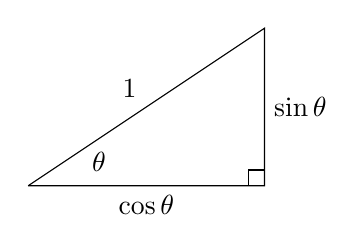
\begin{tikzpicture}[x=10mm, y=10mm]
	\coordinate (A) at (0,0);
	\coordinate (B) at (3,0);
	\coordinate (C) at (3,2);
	\draw (A) -- (B) -- (C) -- (A);
	\draw (B) rectangle ($(B)+(-.2,.2)$);
	\path ($(A)+(.9,.3)$) node [] {$\theta$};
	\path (A) -- (B) node [midway, below] {$\cos\theta$};
	\path (B) -- (C) node [midway, right] {$\sin\theta$};
	\path (A) -- (C) node [midway, above left] {1};
\end{tikzpicture}
\qquad
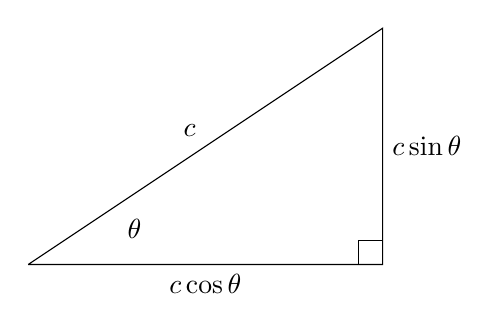
\begin{tikzpicture}[x=15mm, y=15mm]
	\coordinate (A) at (0,0);
	\coordinate (B) at (3,0);
	\coordinate (C) at (3,2);
	\draw (A) -- (B) -- (C) -- (A);
	\draw (B) rectangle ($(B)+(-.2,.2)$);
	\path ($(A)+(.9,.3)$) node [] {$\theta$};
	\path (A) -- (B) node [midway, below] {$c\cos\theta$};
	\path (B) -- (C) node [midway, right] {$c\sin\theta$};
	\path (A) -- (C) node [midway, above left] {$c$};
\end{tikzpicture}
\ 
\begin{tikzpicture}[x=15mm, y=15mm]
	\coordinate (A) at (0,0);
	\coordinate (B) at (4,0);
	\coordinate (C) at (3,2);
	\draw (A) -- (B) -- (C) -- (A);
	\path ($(A)+(.9,.3)$) node [] {$\alpha$};
	\path (A) -- (B) node [midway, below] {$c$};
	\path (B) -- (C) node [midway, above right] {$a$};
	\path (A) -- (C) node [midway, above left] {$b$};
	\node at (A) [below left] {$A$};
	\node at (B) [below right] {$B$};
	\node at (C) [above] {$C$};
\end{tikzpicture}

\

The Law of Cosines says that $a^2 = b^2 + c^2 - 2bc \cos \alpha$.

\

\subsubsection{Derivation of $\vec{u} \cdot \vec{v} = |\vec{u}| |\vec{v}| \cos \theta$}

\

\hfil\begin{tikzpicture}[x=15mm, y=15mm]
	\coordinate (A) at (0,0);
	\coordinate (B) at (4,0);
	\coordinate (C) at (3,2);
	\draw [-triangle 60] (A) -- (B);
	\draw [-triangle 60] (A) -- (C);
	\path ($(A)+(.9,.3)$) node [] {$\theta$};
	\path (A) -- (B) node [midway, below] {$\vec{u} = (a,b,c)$};
	\path (A) -- (C) node [midway, sloped, above] {$\vec{v} = (d,e,f)$};
	\node at (A) [below left] {$(0,0)$};
\end{tikzpicture}

\

Make it a triangle and apply the Law of Cosines.  

\

\hfil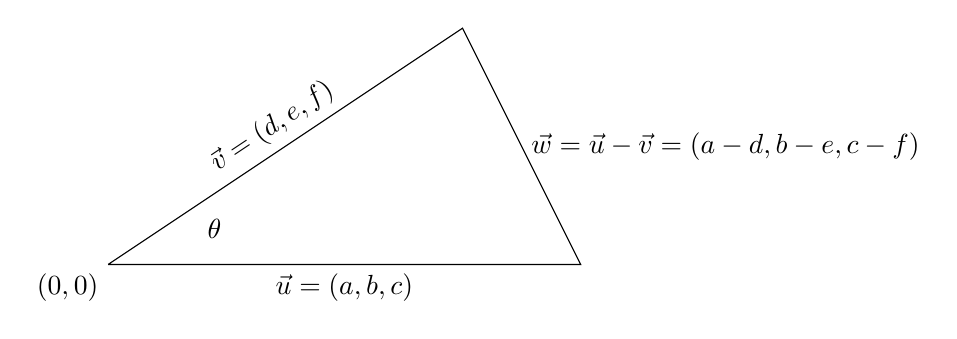
\begin{tikzpicture}[x=15mm, y=15mm]
	\coordinate (A) at (0,0);
	\coordinate (B) at (4,0);
	\coordinate (C) at (3,2);
	\draw (A) -- (B) -- (C) -- (A);
	\path ($(A)+(.9,.3)$) node [] {$\theta$};
	\path (A) -- (B) node [midway, below] {$\vec{u} = (a,b,c)$};
	\path (A) -- (C) node [midway, sloped, above] {$\vec{v} = (d,e,f)$};
	\path (B) -- (C) node [midway, right] {$\vec{w} = \vec{u} - \vec{v} = (a-d,b-e,c-f)$};
	\node at (A) [below left] {$(0,0)$};
\end{tikzpicture}

\

\begin{tabular}{>{$}r<{$}>{$}c<{$}>{$}l<{$\vrule width 0pt height 12pt depth 12pt}}
|\vec{w}|^2 &=& |\vec{u}|^2 + |\vec{v}|^2 - 2 |\vec{u}| |\vec{v}| \cos \theta \cr
(a-d)^2 + (b-e)^2 + (c-f)^2 &=& (a^2 + b^2 + c^2) + (d^2 + e^2 + f^2)   - 2 |\vec{u}| |\vec{v}| \cos \theta \cr
a^2 - 2ad + d^2 + b^2 - 2be + e^2 + c^2 - 2cf + f^2  &=& (a^2 + b^2 + c^2) + (d^2 + e^2 + f^2)   - 2 |\vec{u}| |\vec{v}| \cos \theta \cr
- 2ad - 2be - 2cf &=&   - 2 |\vec{u}| |\vec{v}| \cos \theta \cr
ad + be  + cf &=&    |\vec{u}| |\vec{v}| \cos \theta \cr
\vec{u} \cdot \vec{v} &=&    |\vec{u}| |\vec{v}| \cos \theta \qquad Q.E.D. \cr
\end{tabular}

\

\subsubsection{Dot product as a projection}

\

\begin{tikzpicture}[x=5mm, y=5mm]
	\coordinate (A) at (0,0);
	\coordinate (B) at (8,4);
	\coordinate (C) at (6,12);
	\coordinate (P) at (12,0);
	\coordinate (Q) at (0,8);
	\draw [-triangle 60] (A) -- (B);
	\draw [-triangle 60] (A) -- (C);
	\coordinate (D) at (intersection of A--B and C--P);
	\coordinate (E) at (intersection of A--C and B--Q);
	\path ($1.1*(B)$) node {$\vec{u}$};
	\path ($1.1*(C)$) node {$\vec{v}$};
	\path (A) -- (B) node [midway, below right] {$|\vec{u}|$};
	\path (A) -- (C) node [midway, above left] {$|\vec{v}|$};
	\path (2,2) node {$\theta$};
%	\fill (D) circle (2pt);
%	\fill (E) circle (2pt);
\end{tikzpicture}
\qquad
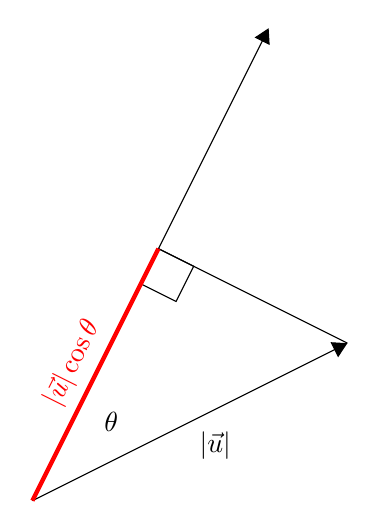
\begin{tikzpicture}[x=5mm, y=5mm]
	\coordinate (A) at (0,0);
	\coordinate (B) at (8,4);
	\coordinate (C) at (6,12);
	\coordinate (P) at (12,0);
	\coordinate (Q) at (0,8);
	\draw [-triangle 60] (A) -- (B);
	\draw [-triangle 60] (A) -- (C);
	\coordinate (D) at (intersection of A--B and C--P);
	\coordinate (E) at (intersection of A--C and B--Q);
%	\path ($1.1*(B)$) node {$\vec{u}$};
%	\path ($1.1*(C)$) node {$\vec{v}$};
	\path (A) -- (B) node [midway, below right] {$|\vec{u}|$};
%	\path (A) -- (C) node [midway, above left] {$|\vec{v}|$};
	\path (2,2) node {$\theta$};
	\draw (A) -- (E) -- (B);
	\draw [rotate={atan(-1/2)}] (E) rectangle ($(E)+(1,-1)$);
	\draw [ultra thick, red] (A) -- (E) node [midway, sloped, above] {$|\vec{u}| \cos \theta$};
%	\fill (D) circle (2pt);
%	\fill (E) circle (2pt);
\end{tikzpicture}
\qquad
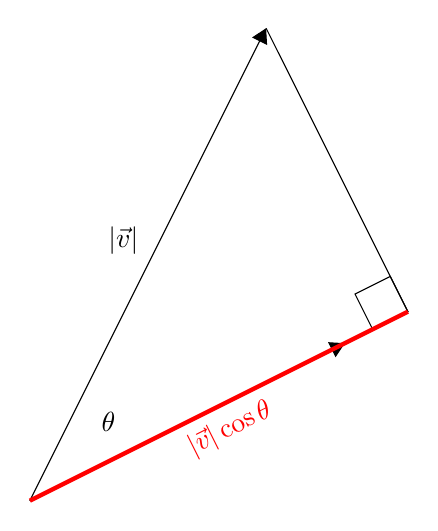
\begin{tikzpicture}[x=5mm, y=5mm]
	\coordinate (A) at (0,0);
	\coordinate (B) at (8,4);
	\coordinate (C) at (6,12);
	\coordinate (P) at (12,0);
	\coordinate (Q) at (0,8);
	\draw [-triangle 60] (A) -- (B);
	\draw [-triangle 60] (A) -- (C);
	\coordinate (D) at (intersection of A--B and C--P);
	\coordinate (E) at (intersection of A--C and B--Q);
%	\path ($1.1*(B)$) node {$\vec{u}$};
%	\path ($1.1*(C)$) node {$\vec{v}$};
%	\path (A) -- (B) node [midway, below right] {$|\vec{u}|$};
	\path (A) -- (C) node [midway, above left] {$|\vec{v}|$};
	\path (2,2) node {$\theta$};
	\draw (A) -- (D) -- (C);
	\draw [rotate={atan(-2)}] (D) rectangle ($(D)+(-1,-1)$);
	\draw [ultra thick, red] (A) -- (D) node [midway, sloped, below] {$|\vec{v}| \cos \theta$};
%	\fill (D) circle (2pt);
%	\fill (E) circle (2pt);
\end{tikzpicture}

\

The segment of length $|\vec{u}| \cos \theta$ is the {\it projection} of $\vec{u}$ onto $\vec{v}$.

The segment of length $|\vec{v}| \cos \theta$ is the {\it projection} of $\vec{v}$ onto $\vec{u}$.

\

In the middle triangle, you can visualize the dot product, $\vec{u} \cdot \vec{v} = |\vec{u}| |\vec{v}| \cos theta$, as the product of the length of the projection onto $\vec{v}$ and the length of $\vec{v}$.  Similarly in the left triangle, you can visualize the dot product as the product of the length of the projection onto $\vec{u}$ and the length of $\vec{u}$.  

\subsection{Cross Product}

\subsubsection{Finding the Cross Product using the Determinant}

The {\it determinant} of a matrix is a scalar that embodies many mysterious properties of the matrix.  

To find the cross product of $\vec{u} = (a,b,c)$ and $\vec{v} = (d,e,f)$, let $\vec{i} = (1,0,0)$, $\vec{j}=(0,1,0)$, and $\vec{k}=(0,0,1)$ be the unit vectors in the $x$, $y$ and $z$ directions.  

$$\vec{u} \times \vec{v} = 
\left|
\begin{tabular}{*3{>{$}l<{$}}}
	\vec{i} & \vec{j} & \vec{k} \cr
	a & b & c \cr
	d & e & f \cr
\end{tabular}
\right|
= 
\left| 
\begin{tabular}{*2{>{$}l<{$}}}
	b & c \cr
	e & f \cr
\end{tabular}
\right|
\vec{i}
\ - \
\left| 
\begin{tabular}{*2{>{$}l<{$}}}
	a & c \cr
	d & f \cr
\end{tabular}
\right|
\vec{j}
\ + \ 
\left| 
\begin{tabular}{*2{>{$}l<{$}}}
	a & b \cr
	d & e\cr
\end{tabular}
\right|
\vec{k}
$$

$$ = (bf-ce)\vec{i} - (af-cd) \vec{j} + (ae-bd)\vec{k} = 
\left[
\begin{tabular}{*3{>{$}l<{$}}}
	bf-ce \cr
	cd-af \cr
	ae-bd
\end{tabular}
\right]
$$

\

The derivation of the identity that the magnitude of the cross product is the product of the magnitudes of the vectors and the sine of the angle between them is to long to fit in the margin of this paper.  

\

I believe it comes from $\displaystyle \cos \theta = \frac{\vec{u} \cdot \vec{v}}{|\vec{u}| |\vec{v}|}$ and $\sin^2 \theta = 1 - \cos^2 \theta$.  

\

\subsubsection{Cross Product as the Area of the Parallelogram}

The area of a parallelogram is base $\times$ height, where the height is perpendicular to the base.  The area of this parallelogram is $|\vec{u}| |\vec{v}| \sin \theta$, which is the magnitude of the cross product.  

\

\hfil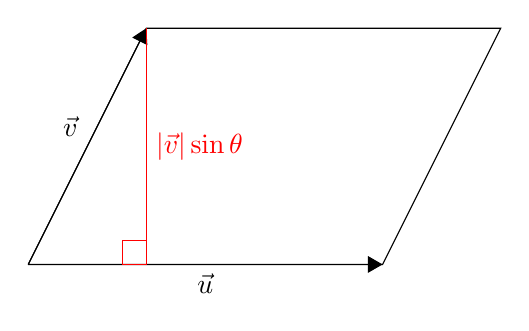
\begin{tikzpicture}[x=15mm, y=15mm]
	\coordinate (A) at (0,0);
	\coordinate (B) at (3,0);
	\coordinate (C) at (1,2);
	\coordinate (D) at (4,2);
	\coordinate (E) at (1,0);
	\draw (A) -- (B) -- (D) -- (C) -- (A);
	\draw [-triangle 60] (A) -- (B);
	\draw [-triangle 60] (A) -- (C);
	\draw [red] (C) -- (E) node [midway, right] {$|\vec{v}|\sin\theta$};
	\draw [red] (E) rectangle (0.8,0.2);
	\path (A) -- (B) node [midway, below] {$\vec{u}$};
	\path (A) -- (C) node [midway, above left] {$\vec{v}$};
\end{tikzpicture}


%%%%%%%%%%%%%%%%
\section{Tuesday 11 September:  Color Models}
%%%%%%%%%%%%%%%%

\subsection{Anti-Aliasing}

Oblique lines of the same length have less color intensity because the pixels are more scattered.  

Anti-aliasing can be performed with greyscale.

Grey level intensity proportional to the area covered.  

Randomizing subpixels (Sampling error)

\subsection{Character Generation}

Bitmap fonts v/s outline fonts

Ideal:  Start with outline fonts, render into font cache.  

\subsection{Color Models}

Parts of a color model:

\begin{itemize}
	\item Hue.  Distinguishes b/n colors, relates to ``dominant wavelength''
	\item Saturation.  How far a color is from grey.  ``Excitation purity.''
	\item Light.  Perceived intensity, reflected.  ``Luminance.''
\end{itemize}

Humans are less sensitive to variations in blue than variations in red or green.  

\subsubsection{RGB:  ``Emitting Light''}

RGB is device-oriented.  

\

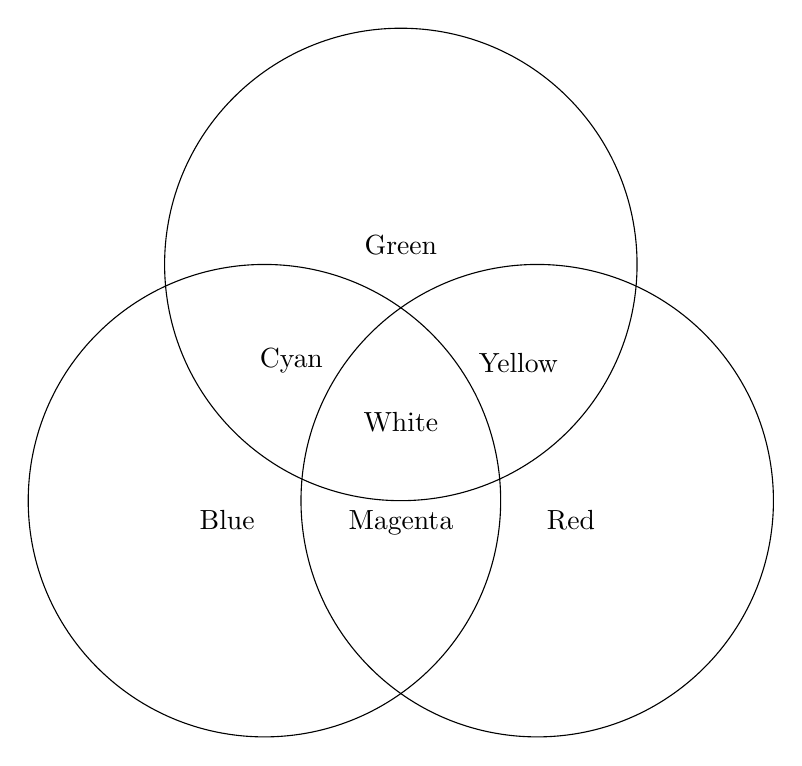
\begin{tikzpicture}[x=20mm,y=20mm]
	\coordinate (G) at ({cos(90)},{sin(90)});
	\coordinate (B) at ({cos(210)},{sin(210)});
	\coordinate (R) at ({cos(330)},{sin(330)});
	\coordinate (C) at ({0.5*cos(150)},{0.5*sin(150)});
	\coordinate (M) at ({0.5*cos(270)},{0.5*sin(270)});
	\coordinate (Y) at ({0.5*cos(30)},{0.5*sin(30)});
	\draw (G) circle (1.5);
	\draw (B) circle (1.5);
	\draw (R) circle (1.5);
	\path (G) node [above] {Green};
	\path (B) node [below left] {Blue};
	\path (R) node [below right] {Red};
	\path (C) node [above left] {Cyan};
	\path (M) node [below] {Magenta};
	\path (Y) node [above right] {Yellow};
	\path (0,0) node [] {White};
\end{tikzpicture}

There is no wavelength that gives ``magenta.'' We perceive it as one color, even though it is the mixture of two colors.  

\subsubsection{RGB Cube}

\tdplotsetmaincoords{70}{110}
\begin{tikzpicture}[scale=5,tdplot_main_coords]

%set up some coordinates 
%-----------------------
\coordinate (O) at (0,0,0);
\coordinate (R) at (0,0,1);
\coordinate (G) at (0,1,0);
\coordinate (B) at (1,0,0);
\coordinate (M) at (1,0,1);
\coordinate (C) at (1,1,0);
\coordinate (Y) at (0,1,1);
\coordinate (W) at (1,1,1);

\draw[thick,->] (O) -- ($1.2*(B)$) node[anchor=north east]{B};
\draw[thick,->] (O) -- ($1.2*(G)$) node[anchor=north west]{G};
\draw[thick,->] (O) -- ($1.2*(R)$) node[anchor=south]{R};

\draw (R) -- (M) -- (B) -- (C) -- (G) -- (Y) -- (R);
\draw (C) -- (W);
\draw (M) -- (W);
\draw (Y) -- (W);

\path (O) node [above right] {Black};
\path (W) node [below left] {White};
\path (C) node [below] {Cyan};
\path (M) node [left] {Magenta};
\path (Y) node [right] {Yellow};



%\foreach \i in {0, 30, 60, ..., 360}{
%	\foreach \j in {0, 0.2, 0.4,...,1}{
%		\draw (\j, {cos(\i)*0.2},{sin(\i)*.2)}) -- (\j, {cos(\i+30)*0.2},{sin(\i+30)*.2)}); 
%	}
%}

\end{tikzpicture}


\subsubsection{CMY:  ``Absorbing Light.''}

Printers use CMY (Cyan, Magenta, Yellow)

$$
\left[
	\begin{array}{c}
		\text{C} \cr
		\text{M} \cr
		\text{Y} \cr
	\end{array}
\right]
=
\left[
	\begin{array}{c}
		\text{1} \cr
		\text{1} \cr
		\text{1} \cr
	\end{array}
\right]
-
\left[
	\begin{array}{c}
		\text{R} \cr
		\text{G} \cr
		\text{B} \cr
	\end{array}
\right]
$$

\subsubsection{HSV Model}

Hue, Saturation, Value

Cone shaped

More artist-oriented.  

\subsection{Modeling the World}

Surface modeling, Materials properties, Scene graph organization

Surface representation techniques:  

\qquad Polygon meshes

\qquad Triangle meshes (in this class)

Polygon rendering:

\qquad Consider each polygon

\qquad Project onto a 2D viewing screen.  



%%%%%%%%%%%%%%
\section{Thursday 13 September:  Triangle Mesh}
%%%%%%%%%%%%%

HW \#2 Triangle Mesh

Move around based on user clicks.  

\

Primitive called OpenGL Triangle Strip

\

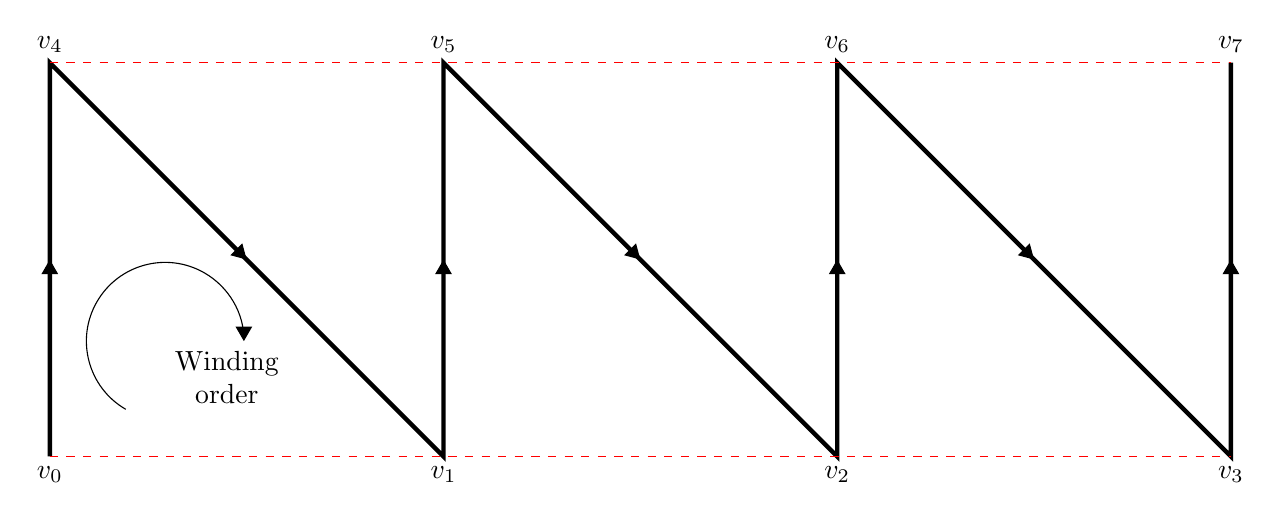
\begin{tikzpicture}[x=50mm, y=50mm]
	\coordinate (v0) at (0,0);
	\coordinate (v1) at (1,0);
	\coordinate (v2) at (2,0);
	\coordinate (v3) at (3,0);
	\coordinate (v4) at (0,1);
	\coordinate (v5) at (1,1);
	\coordinate (v6) at (2,1);
	\coordinate (v7) at (3,1);
	\path (v0) node [below] {$v_0$};
	\path (v1) node [below] {$v_1$};
	\path (v2) node [below] {$v_2$};
	\path (v3) node [below] {$v_3$};
	\path (v4) node [above] {$v_4$};
	\path (v5) node [above] {$v_5$};
	\path (v6) node [above] {$v_6$};
	\path (v7) node [above] {$v_7$};
	\draw [ultra thick] (v0) -- (v4) -- (v1) -- (v5) -- (v2) -- (v6) -- (v3) -- (v7);
	\draw [-triangle 60] (v0) -- ($0.5*(v0)+0.5*(v4)$);
	\draw [-triangle 60] (v4) -- ($0.5*(v4)+0.5*(v1)$);
	\draw [-triangle 60] (v1) -- ($0.5*(v1)+0.5*(v5)$);
	\draw [-triangle 60] (v5) -- ($0.5*(v5)+0.5*(v2)$);
	\draw [-triangle 60] (v2) -- ($0.5*(v2)+0.5*(v6)$);
	\draw [-triangle 60] (v6) -- ($0.5*(v6)+0.5*(v3)$);
	\draw [-triangle 60] (v3) -- ($0.5*(v3)+0.5*(v7)$);
	\draw [dashed, red] (v0) -- (v3);
	\draw [dashed, red] (v4) -- (v7);
	\coordinate (C) at (${sqrt(2)/(2+sqrt(2))}*(v0)+{1/(2+sqrt(2))}*(v1)+{1/(2+sqrt(2))}*(v4)$);
	\draw [-triangle 60] ($(C)+({0.2*cos(240)},{0.2*sin(240)})$) arc (240:0:0.2);
	\path (C) node [below right, align=center] {Winding \\ order};
	\coordinate (D) at (${sqrt(2)/(2+sqrt(2))}*(v5)+{1/(2+sqrt(2))}*(v1)+{1/(2+sqrt(2))}*(v4)$);
%	\draw [triangle 60-] ($(D)+({0.2*cos(60)},{0.2*sin(60)})$) arc (60:-210:0.2);
\end{tikzpicture}

\

Dr. Borst's Annotation:  Note about winding order: it is the first triangle in the strip that determines the winding order for all triangles in the strip. so, here we see everything as clockwise. The default is that we want counterclockwise order when viewing the front (or outside) surface. The way I set up the description has us looking at the other side (back/inside) in the ``unwrapped'' mesh diagrams.

\

{\it Vertex List} \quad Array with vertices or vertex array.

$\{ \{ x_0, y_0, z_0 \}, \{ x_1, y_1, z_1\}, \dots, \{x_7, y_7, z_7\}\}$

\

{\it Index List} \quad Order in which the vertices form triangles.

First three vertices define first triangle, next vertex creates another triangle.  

$\{0,4,1,5,2,6,3,7\}$

\

Vertex list gives {\it geometry}, index list gives {\it topology} -- connectivity with neighbors.

\begin{tikzpicture}[x=9mm, y=10mm]
	\clip (-7,-4.1) rectangle (13,4.1);
	\coordinate (A) at (-5,2);
	\coordinate (B) at (-5,-2);
	\coordinate (C) at (5,2);
	\coordinate (D) at (5,-2);
	\coordinate (E) at (-5,0);
	\coordinate (F) at (5,0);
	\coordinate (G) at (5,4);
	\coordinate (H) at (5,-4);
	\coordinate (I) at (10,0);
	\draw (E) ellipse (1 and 2);
	\draw (F) ellipse (1 and 2);
	\draw [name path=ellipse] (F) ellipse (2 and 4);
	\path [name path=oline] (I) -- ({10-1.1*sqrt(21)},{1.1*4});
	\path [name intersections={of = ellipse and oline}];
	\coordinate (J) at (intersection-1);
	\coordinate (K) at (intersection-2);
	\path [name path=nline] (I) -- ({10-1.1*sqrt(21)},-{1.1*4});
	\path [name intersections={of = ellipse and nline}];
	\coordinate (L) at (intersection-1);
	\coordinate (M) at (intersection-2);
	\fill [white] (C) rectangle ($(C)+(-3,-4)$);
	\draw (A) -- (C);
	\draw (B) -- (D);
	\draw (J) -- (I) -- (L);
	\draw [dashed, triangle 60-triangle 60] (-5,3) -- (-5,0) -- (12,0);
	\path (-5,3) node [above] {$y$};
	\path (12,0) node [right] {$x$};
\end{tikzpicture}

\

\begin{tikzpicture}[x=9mm, y=10mm]
	\clip (-7,-4.1) rectangle (13,4.1);
	\draw [-triangle 60, dashed] (-5,0) -- (12,0);
	\draw [-triangle 60, dashed] (-5,0) -- (-5,2);
	\draw (-6,0) circle (0pt);
	\coordinate (A) at (-5,0);
	\coordinate (B) at (-5,-2);
	\coordinate (C) at (5,-2);
	\coordinate (D) at (5,-4);
	\coordinate (E) at (10,0);
	\draw (A) -- (B) -- (C) -- (D) -- (E);
	\path (A) node [left] {${(x_0,y_0)}$};
	\path (B) node [below left] {$(x_1,y_1)$};
	\path (C) node [below left] {$(x_2,y_2)$};
	\path (D) node [below] {$(x_3,y_3)$};
	\path (E) node [below right] {$(x_4,y_4)$};
	\path (-5,3) node [above] {$y$};
	\path (12,0) node [right] {$x$};
\end{tikzpicture}

\

Rotate about $x$-axis.  

\

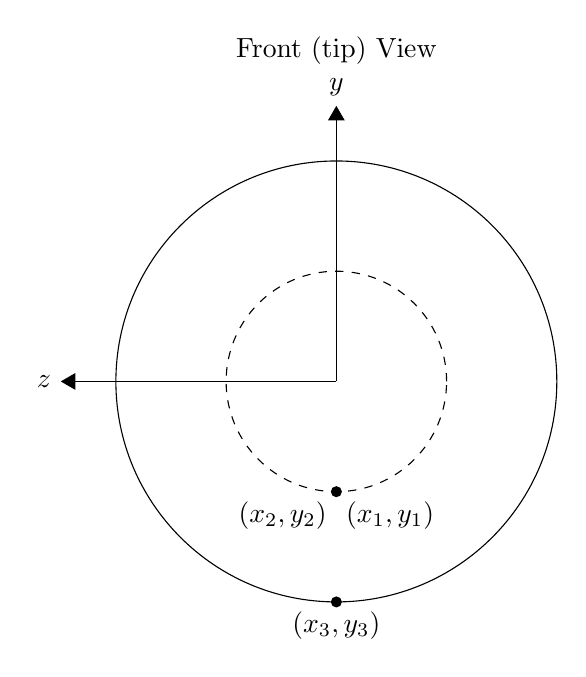
\begin{tikzpicture}[x=7mm, y=7mm]
	\draw [-triangle 60] (0,0) -- (0,5) node [above] {$y$};
	\draw [-triangle 60] (0,0) -- (-5,0) node [left] {$z$};
	\draw (0,0) circle (4);
	\draw [dashed] circle (2);
	\fill (0,-2) circle (2pt);
	\fill (0,-4) circle (2pt);
	\path (0,-2) node [below right] {$(x_1,y_1)$};
	\path (0,-2) node [below left] {$(x_2,y_2)$};
	\path (0,-4) node [below] {$(x_3,y_3)$};
	\path (0,6) node {Front (tip) View};
\end{tikzpicture}
\hfill
\begin{tikzpicture}[x=7mm, y=7mm]
	\draw [-triangle 60] (0,0) -- (0,5) node [above] {$y$};
	\draw [-triangle 60] (0,0) -- (-5,0) node [left] {$z$};
	\draw (0,0) circle (4);
	\coordinate (A) at (0,0);
	\coordinate (B) at ({4*cos(330)},{4*sin(330)});
	\coordinate (C) at (0,{4*sin(330)});
	\draw (A) -- (B) -- (C) -- (A);
	\fill (0,-4) circle (2pt) node [below] {$(x_{i0},y_{i0}, 0)$};
	\fill (B) circle (2pt) node [below right] {$(x_{i0}, y_{i0} \cos \theta, y_{i0} \sin \theta)$};
	\draw (C) rectangle ($(C)+(0.3,0.3)$);
	\path (B) -- (C) node [ midway, below] {$y_{i0} \sin \theta$};
	\path (A) -- (C) node [ midway, left] {$y_{i0} \cos \theta$};
	\path (A) -- (B) node [ midway, above] {$y_{i0}$};
	\path ({1*cos(300)},{1*sin(300)})  node {$\theta$};
\end{tikzpicture}


\

Positive rotation is counter-clockwise when the axis is pointing towards you.  

\

Let $np$ be the number of points to be rotated, and $nm$ be the number of steps of the rotation.  Note that there will be $nm+1$ copies of the profile, with the last one being at $\theta = 2\pi$, duplicating the vertices at $\theta = 0$, closing the loop.  

\

Vertex list:  

\qquad $(x_{ij}, y_{ij}, z_{ij}) = (x_{i0}, \cos \theta y_{i0}, \sin\theta y_{i0})$ with $\displaystyle\theta = \frac{2\pi}{nm} j$ for $0 \le i < np$ and  $0 \le j \le nm$.


\

\subsection{Array of a Rotated Surface}

The bottom and top rows are the same.  

Vertical lines represent different $x$ values.  More strictly speaking, vertical lines correspond to different $i$ values, but could actually repeat $x$ (not necessarily different x values) as in the first two points of the drawn arrow.

Horizontal lines represent different values of $\theta$.  

\

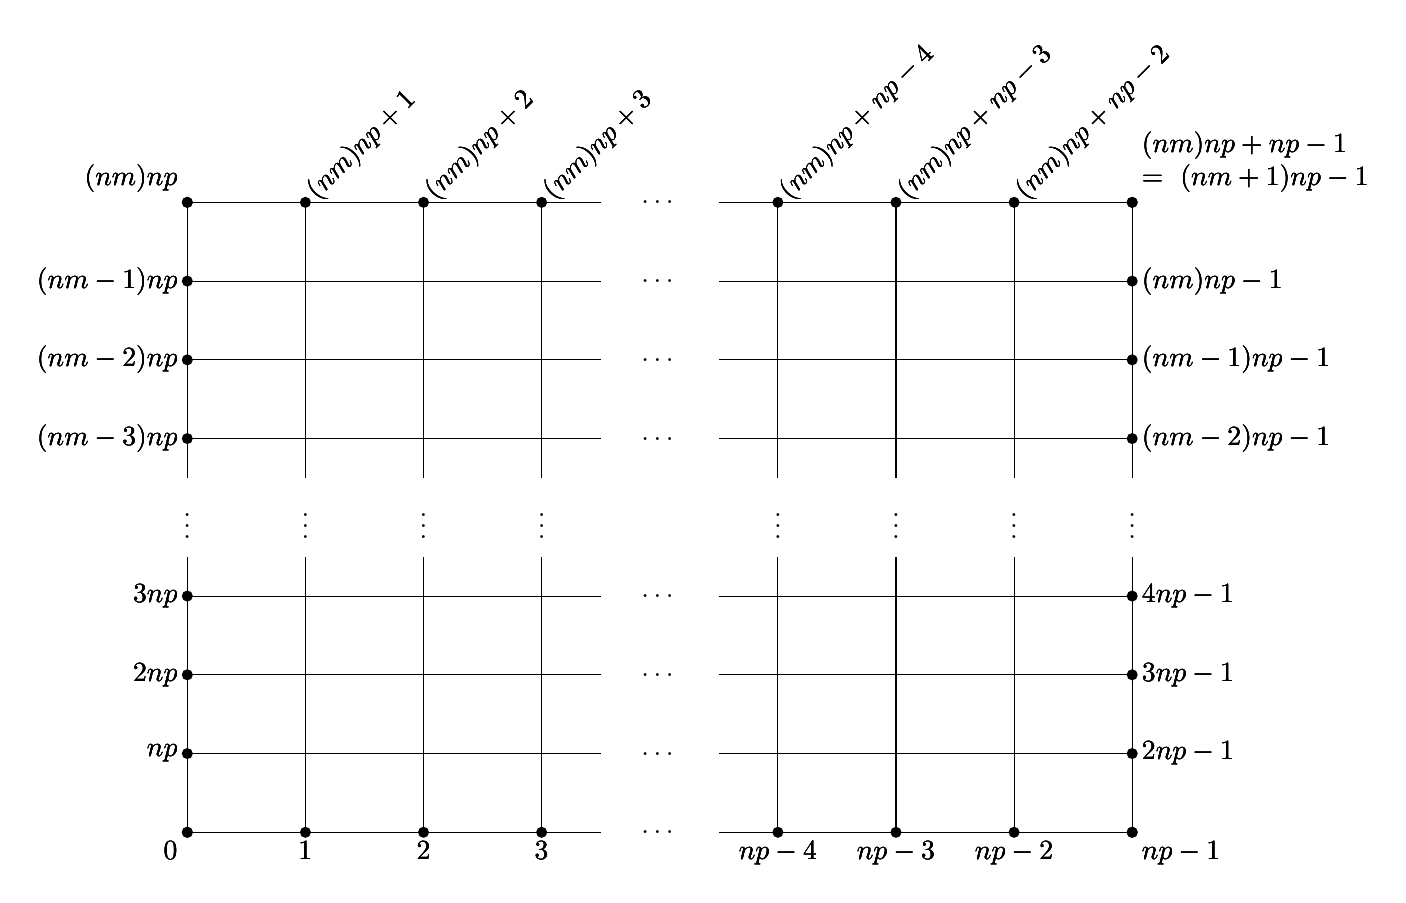
\begin{tikzpicture}[x=15mm,y=10mm]
	\foreach \i in {0,1,2,3}{
		% Lower left
		\draw (0,\i) -- (3.5, \i);
		\draw (\i,0) -- (\i,3.5);
		\path (\i,4) node {$\vdots$};
		\path (4,\i) node {$\dots$};
		\fill (0,\i) circle (2pt);
		\fill (\i,0) circle (2pt);
		% Upper left
		\draw (\i,4.5) -- (\i,8);
		\draw (0,{\i+5}) -- (3.5,{\i+5}); 
		\path (4,{\i+5}) node {$\dots$};
		\fill (0,{\i+5}) circle (2pt);
		\fill (\i,8) circle (2pt);
		% Lower right
		\draw ({\i+5},0) -- ({\i+5},3.5);
		\draw (4.5,{\i}) -- (8,{\i}); 
		\path ({\i+5},4) node {$\vdots$};
		\fill ({\i+5},0) circle (2pt);
		\fill (8, {\i}) circle (2pt);
		% Upper right
		\draw ({\i+5},4.5) -- ({\i+5},8);
		\draw (4.5,{\i+5}) -- (8,{\i+5}); 
		\fill ({\i+5},8) circle (2pt);
		\fill (8,{\i+5}) circle (2pt);
		\path (0,0) node [below left] {$0$};
		\path (1,0) node [below] {$1$};
		\path (2,0) node [below] {$2$};
		\path (3,0) node [below] {$3$};
		\path (5,0) node [below] {$np-4$};
		\path (6,0) node [below] {$np-3$};
		\path (7,0) node [below] {$np-2$};
		\path (8,0) node [below right] {$np-1$};
		\path (0,1) node [left] {$np$};
		\path (0,2) node [left] {$2np$};
		\path (0,3) node [left] {$3np$};
		\path (0,5) node [left] {$(nm-3)np$};
		\path (0,6) node [left] {$(nm-2)np$};
		\path (0,7) node [left] {$(nm-1)np$};
		\path (0,8) node [above left] {$(nm)np$};
		\path (8,1) node [right] {$2np-1$};
		\path (8,2) node [right] {$3np-1$};
		\path (8,3) node [right] {$4np-1$};
		\path (8,5) node [right] {$(nm-2)np - 1$};
		\path (8,6) node [right] {$(nm-1)np - 1$};
		\path (8,7) node [right] {$(nm)np - 1$};
		\path (8,8) node [above right, align=left] {$(nm)np + np - 1$ \\ $= \ (nm+1)np - 1$};
		\path (1,8) node [rotate=45, right] {$(nm)np + 1$};
		\path (2,8) node [rotate=45, right] {$(nm)np + 2$};
		\path (3,8) node [rotate=45, right] {$(nm)np + 3$};
		\path (5,8) node [rotate=45, right] {$(nm)np + np-4$};
		\path (6,8) node [rotate=45, right] {$(nm)np + np-3$};
		\path (7,8) node [rotate=45, right] {$(nm)np + np-2$};
%		\path (,8) node [above, rotate=45] {$$};
%		\path (0,) node [left] {$$};
	}
	
\end{tikzpicture}

How many vertices?  $np\times (nm+1)$

How many cells? $(np-1)(nm)$

How many triangles? $2(np-1)(nm)$

\

Vertex List 

{\tt loop over theta}

\qquad {\tt loop over x}

\

{\tt for theta in range (nm+1):}

\qquad {\tt for i in range (np):}

\qquad \qquad {\tt x(x,theta), y(x,theta), z(x,theta)}

\

{\color{red}  I have this in my notes, but I think it's wrong. 

$\{ 
	x_{0,0}, y_{0,0}, z_{0,0},
	x_{0,1}, y_{0,1}, z_{0,1},
$
}

\

$\{ 
	x_{0,0}, y_{0,0}, z_{0,0},
	x_{1,0}, y_{1,0}, z_{1,0},
	\dots,
	x_{np-1,0}, y_{np-1,0}, z_{np-1,0},
$

\qquad$
	x_{0,1}, y_{0,1}, z_{0,1},
	\dots,
$

\qquad \qquad $
	\dots, x_{np-1,nm}, y_{np-1,nm}, z_{np-1,nm},
\}$

\

Index List, using {\it primitive restart index}

$\{ 0, np, 1, np+1, 2, np+2, \dots, np-1, 2np-1, $ restart,

$np, 2np, np+1, 2np+1, \dots, 2np-2, 3np-2, 2np-2, 3np-1,$ restart,

$\vdots$

$(nm-1)np, (nm)np, (nm-1)np + 1, (nm)np+1, \dots, (nm)np-1, (nm+1)np - 1$, restart $\}$








\section{Tuesday 18 September:  Translations}

\subsection{Introduction}

\tdplotsetmaincoords{70}{110}
\begin{tikzpicture}[scale=1,tdplot_main_coords]

%set up some coordinates 
%-----------------------
\coordinate (O) at (0,0,0);
\coordinate (p1) at (0,1,0);
\coordinate (p2) at (4,1,0);
\coordinate (p3) at (4,2,0);
\coordinate (p4) at (6,0,0);
\draw [red] (O) -- (p1) -- (p2) -- (p3) -- (p4);

\draw[thick,->] (O) -- (8,0,0) node[anchor=north east]{$x$};
\draw[thick,->] (O) -- (0,3,0) node[anchor=north west]{$y$};
\draw[thick,->] (O) -- (0,0,3) node[anchor=south]{$z$};

\foreach \i in {0,60,...,360}{
	\draw [red, dashed] (0,0,0)
		 -- (0,{1*cos(\i)},{1*sin(\i)}) 
		 -- (4,{1*cos(\i)},{1*sin(\i)}) 
		 -- (4,{2*cos(\i)},{2*sin(\i)}) 
		 -- (6,0,0); 
}

\tdplotsetrotatedcoords{60}{40}{-20}
    \coordinate (Shift) at (3,5,4);
    \tdplotsetrotatedcoordsorigin{(Shift)}
\draw [red,tdplot_rotated_coords] (0,0,0) -- (0,1,0) -- (4,1,0) -- (4,2,0) -- (6,0,0);
\draw[thick,color=blue,tdplot_rotated_coords,->] (0,0,0) --
        (2,0,0) node[anchor=north]{$x'$};
    \draw[thick,color=blue,tdplot_rotated_coords,->] (0,0,0) --
        (0,2,0) node[anchor=west]{$y'$};
    \draw[thick,color=blue,tdplot_rotated_coords,->] (0,0,0) --
        (0,0,2) node[anchor=south]{$z'$};
        
\foreach \i in {0,90,...,360}{
	\draw [red, dashed,tdplot_rotated_coords] (0,0,0)
		 -- (0,{1*cos(\i)},{1*sin(\i)}) 
		 -- (4,{1*cos(\i)},{1*sin(\i)}) 
		 -- (4,{2*cos(\i)},{2*sin(\i)}) 
		 -- (6,0,0); 
}

\path (6,2,-2) node {$\{W\}$ World, global coordinate system, global frame};
\path (6,6,-2.5) node [blue] {$\{L\}$ Local coordinate system, Local frame};

\end{tikzpicture}

$\displaystyle ^{W}_{L}M$ is the matrix transformation ``$\{L\}$ with respect to $\{W\}$'', or just ``$\{L\}$ to $\{W\}$.''  

\qquad is a description of $\{L\}$ with respect to $\{W\}$.

\qquad is a matrix that converts a point in $\{L\}$ to a point in $\{W\}$.

\qquad \qquad $\displaystyle ^{W}P = ^W_LM ^LP$

\qquad is an operation that moves an object.  

\

\subsection{Conventions}

Right-handed frames (coordinate systems)

Points written as column vectors.  If row vectors, the matrices have to be transposed and the order of multiplication reversed.  

\

{\bf Transformations}  Translation, Rotation, and Scale

\subsection{Translation: Change in Position}

$P' = P + T$
\qquad
$\displaystyle 
\left[
\begin{array}{c}
	x' \cr
	y' \cr
	z' \cr
\end{array}
\right] 
=
\left[
\begin{array}{c}
	x \cr
	y \cr
	z \cr	
\end{array}
\right] 
+
\left[
\begin{array}{c}
	t_x \cr
	t_y \cr
	t_z \cr	
\end{array}
\right] 
$

\tdplotsetmaincoords{70}{110}
\begin{tikzpicture}[scale=1,tdplot_main_coords]

%set up some coordinates 
%-----------------------
\coordinate (O) at (0,0,0);
\coordinate (p1) at (0,1,0);
\coordinate (p2) at (4,1,0);
\coordinate (p3) at (4,2,0);
\coordinate (p4) at (6,0,0);
\draw [red] (O) -- (p1) -- (p2) -- (p3) -- (p4);

\draw[thick,->] (O) -- (8,0,0) node[anchor=north east]{$x$};
\draw[thick,->] (O) -- (0,3,0) node[anchor=north west]{$y$};
\draw[thick,->] (O) -- (0,0,3) node[anchor=south]{$z$};

\tdplotsetrotatedcoords{0}{0}{0}
    \coordinate (Shift) at (3,5,4);
    \tdplotsetrotatedcoordsorigin{(Shift)}
\draw [red,tdplot_rotated_coords] (0,0,0) -- (0,1,0) -- (4,1,0) -- (4,2,0) -- (6,0,0);
\draw[thick,color=blue,tdplot_rotated_coords,->] (0,0,0) --
        (2,0,0) node[anchor=north]{$x'$};
    \draw[thick,color=blue,tdplot_rotated_coords,->] (0,0,0) --
        (0,2,0) node[anchor=west]{$y'$};
    \draw[thick,color=blue,tdplot_rotated_coords,->] (0,0,0) --
        (0,0,2) node[anchor=south]{$z'$};
        

\end{tikzpicture}

\

Apply transform to every point in the mesh.  

\

OpenGL note:  Pass $M$ to the graphics system.  $M$ is applied to the vertex shader.  

We will get a {\it vertex shader}, but we will have to load it in the graphics card.  

\

\subsection{Scale:  Change in size}

$\displaystyle P' = SP
\qquad
\left[
\begin{array}{c}
	x' \cr
	y' \cr
	z' \cr
\end{array}
\right] 
= 
\left[
\begin{array}{ccc}
	s_x & 0 & 0 \cr
	0 & s_y & 0 \cr
	0 & 0 & s_z \cr	
\end{array}
\right] 
\left[
\begin{array}{c}
	x \cr
	y \cr
	z \cr	
\end{array}
\right] 
=
\left[
\begin{array}{c}
	s_x x \cr
	s_y y \cr
	s_z z \cr	
\end{array}
\right] 
$

\

In {\it uniform scale}, the three scale factors are the same.  

\vskip -1in
\tdplotsetmaincoords{70}{110}
\hfill\begin{tikzpicture}[scale=1,tdplot_main_coords]

%set up some coordinates 
%-----------------------
\coordinate (O) at (0,0,0);
\coordinate (p1) at (0,1,0);
\coordinate (p2) at (4,1,0);
\coordinate (p3) at (4,2,0);
\coordinate (p4) at (6,0,0);
\draw [red] (O) -- (p1) -- (p2) -- (p3) -- (p4);
\draw [red, dashed] (O) -- ($1.2*(p1)$) -- ($1.2*(p2)$) -- ($1.2*(p3)$) -- ($1.2*(p4)$);

\draw[thick,->] (O) -- (8,0,0) node[anchor=north east]{$x$};
\draw[thick,->] (O) -- (0,3,0) node[anchor=north west]{$y$};
\draw[thick,->] (O) -- (0,0,3) node[anchor=south]{$z$};


\end{tikzpicture}

\subsection{Rotation:  Change in Orientation}

Later in the class we'll talk more about rotation.

Example:  Rotation of $\theta$ about the $z$-axis. 

\qquad Values of $z$ do not change. 

\

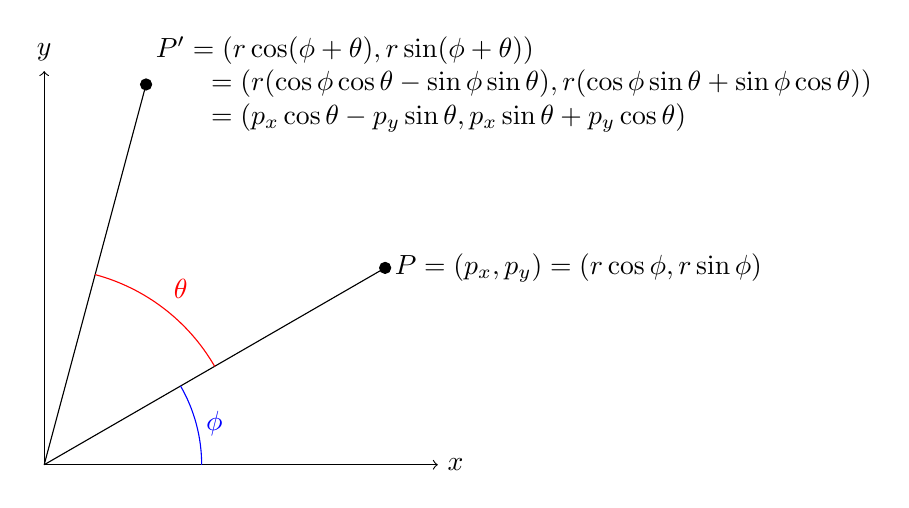
\begin{tikzpicture}[x=50mm, y=50mm]
	\draw [->] (0,0) -- (0,1) node [above] {$y$};
	\draw [->] (0,0) -- (1,0) node [right] {$x$};
	\filldraw (0,0) -- ({cos(30)},{sin(30)}) circle (2pt) node [right] {$P = (p_x, p_y) = (r \cos \phi, r\sin\phi)$};
	\filldraw (0,0) -- ({cos(75)},{sin(75)}) circle (2pt) node [right, align=left] {$P' = (r \cos (\phi + \theta),r\sin(\phi+\theta))$ 
	\\ \qquad  $= (r(\cos \phi \cos \theta - \sin \phi \sin \theta), r(\cos \phi \sin \theta + \sin \phi \cos \theta))$
	\\ \qquad  $= (p_x \cos \theta - p_y \sin \theta, p_x \sin\theta + p_y \cos \theta)$
	};
	\draw [blue] ({0.4*cos(0)},{0.4*sin(0)}) arc (0:30:0.4) node [midway, right] {$\phi$};
	\draw [red] ({0.5*cos(30)},{0.5*sin(30)}) arc (30:75:0.5) node [midway, above right] {$\theta$};
\end{tikzpicture}

\

$\displaystyle P' = R \cdot P$
\qquad 
$\displaystyle
\left[
\begin{array}{c}
	p'_x \cr
	p'_y \cr
	p'_z \cr
\end{array}
\right] 
=
\left[
\begin{array}{ccc}
	p_x \cos \theta - p_y \sin \theta \cr
	p_x \sin \theta + p_y \cos \theta \cr
	p_z
\end{array}
\right] 
= 
\left[
\begin{array}{ccc}
	\cos \theta & -\sin\theta & 0 \cr
	\sin \theta & \cos \theta & 0 \cr
	0 & 0 & 1 \cr
\end{array}
\right] 
\left[
\begin{array}{c}
	p_x \cr
	p_y \cr
	p_z \cr	
\end{array}
\right] 
$


\tdplotsetmaincoords{70}{110}
\begin{tikzpicture}[scale=1,tdplot_main_coords]

%set up some coordinates 
%-----------------------
\coordinate (O) at (0,0,0);
\coordinate (p1) at (0,1,0);
\coordinate (p2) at (4,1,0);
\coordinate (p3) at (4,2,0);
\coordinate (p4) at (6,0,0);
\draw [red] (O) -- (p1) -- (p2) -- (p3) -- (p4);

\draw[thick,->] (O) -- (8,0,0) node[anchor=north east]{$x$};
\draw[thick,->] (O) -- (0,3,0) node[anchor=north west]{$y$};
\draw[thick,->] (O) -- (0,0,3) node[anchor=south]{$z$};

\tdplotsetrotatedcoords{0}{0}{30}
    \coordinate (Shift) at (0,0,0);
    \tdplotsetrotatedcoordsorigin{(Shift)}
\draw [blue, dashed ,tdplot_rotated_coords] (0,0,0) -- (0,1,0) -- (4,1,0) -- (4,2,0) -- (6,0,0);
\draw[thick,color=blue,tdplot_rotated_coords,->] (0,0,0) --
        (2,0,0) node[anchor=north]{$x'$};
    \draw[thick,color=blue,tdplot_rotated_coords,->] (0,0,0) --
        (0,2,0) node[anchor=west]{$y'$};
    \draw[thick,color=blue,tdplot_rotated_coords,->] (0,0,0) --
        (0,0,2) node[anchor=south]{$z'$};
        

\end{tikzpicture}

\subsection{Homogeneous Coordinates and Transforms}

Add $w$ coordinate.  For now, $w=1$.
\qquad 
$\displaystyle
\left[
\begin{array}{c}
	x \cr
	y \cr
	z \cr 
	w \cr	
\end{array}
\right] 
$
represents 
$\displaystyle
\left[
\begin{array}{c}
	x/w \cr
	y/w \cr
	z/w \cr 
\end{array}
\right] 
$

\

Dividing by $w$ is called {\it homogenizing the coordinate}.

\subsubsection{Translation}

$\displaystyle
P' = T\cdot P
\qquad
\left[
\begin{array}{c}
	p'_x \cr
	p'_y \cr
	p'_z \cr
	p'_w \cr	
\end{array}
\right] 
= 
\left[
\begin{array}{cccc}
	1 & 0 & 0 & t_x \cr
	0 & 1 & 0 & t_y \cr
	0 & 0 & 1 & t_z \cr
	0 & 0 & 0 & 1 \cr
\end{array}
\right] 
\left[
\begin{array}{c}
	p_x \cr
	p_y \cr
	p_z \cr
	p_w \cr	
\end{array}
\right] 
=
\left[
\begin{array}{c}
	p_x + t_x \cr
	p_y + t_y \cr
	p_z + t_z \cr
	p_w \cr	
\end{array}
\right] 
$

\vskip 24pt

Inverse of $T$, 
$\displaystyle
T^{-1} = 
\left[
\begin{array}{cccc}
	1 & 0 & 0 & -t_x \cr
	0 & 1 & 0 & -t_y \cr
	0 & 0 & 0 & -t_z \cr
	0 & 0 & 0 & 1 \cr
\end{array}
\right] 
$

\subsubsection{Rotation of $\theta$ about the $z$-axis}

$\displaystyle
R = \left[
\begin{array}{cccc}
	\cos \theta & -\sin \theta & 0 & 0 \cr
	\sin \theta & \cos \theta & 0 & 0 \cr
	0 & 0 & 1 & 0 \cr
	0 & 0 & 0 & 1 \cr
\end{array}
\right] 
$

\vskip 24pt


$\displaystyle
R^{-1} = \left[
\begin{array}{cccc}
	\cos (-\theta) & -\sin (-\theta) & 0 & 0 \cr
	\sin (-\theta) & \cos (-\theta) & 0 & 0 \cr
	0 & 0 & 1 & 0 \cr
	0 & 0 & 0 & 1 \cr
\end{array}
\right] 
= 
\left[
\begin{array}{cccc}
	\cos \theta & \sin \theta & 0 & 0 \cr
	-\sin \theta & \cos \theta & 0 & 0 \cr
	0 & 0 & 1 & 0 \cr
	0 & 0 & 0 & 1 \cr
\end{array}
\right] 
= R^T
$

\subsubsection{Scale}

$\displaystyle
S = 
\left[
\begin{array}{cccc}
	s_x & 0 & 0 & 0 \cr
	0 & s_y & 0 & 0 \cr
	0 & 0 &  s_z &	0 \cr
	0 & 0 & 0 & 1 \cr
\end{array}
\right] 
$
\qquad
$\displaystyle
S^{-1} = 
\left[
\begin{array}{cccc}
	1/s_x & 0 & 0 & 0 \cr
	0 & 1/s_y & 0 & 0 \cr
	0 & 0 &  1/s_z &	0 \cr
	0 & 0 & 0 & 1 \cr	
\end{array}
\right] 
$
\quad (for nonzero scaling factors)

\subsection{World v/s Local Translations}

\tdplotsetmaincoords{70}{110}
\begin{tikzpicture}[scale=1,tdplot_main_coords]

%set up some coordinates 
%-----------------------
\coordinate (O) at (0,0,0);
\coordinate (p1) at (0,1,0);
\coordinate (p2) at (4,1,0);
\coordinate (p3) at (4,2,0);
\coordinate (p4) at (6,0,0);
\draw [red] (O) -- (p1) -- (p2) -- (p3) -- (p4);

\draw[thick,->] (O) -- (8,0,0) node[anchor=north east]{$x$};
\draw[thick,->] (O) -- (0,3,0) node[anchor=north west]{$y$};
\draw[thick,->] (O) -- (0,0,3) node[anchor=south]{$z$};

\tdplotsetrotatedcoords{0}{0}{30}
    \coordinate (Shift) at (0,0,0);
    \tdplotsetrotatedcoordsorigin{(Shift)}
\draw [blue, tdplot_rotated_coords] (0,0,0) -- (0,1,0) -- (4,1,0) -- (4,2,0) -- (6,0,0);
\draw [violet, tdplot_rotated_coords] (7,0,0) -- (7,1,0) -- (11,1,0) -- (11,2,0) -- (13,0,0);
\draw[thick,color=blue,tdplot_rotated_coords,->] (0,0,0) --
        (2,0,0) node[anchor=north]{$x'$};
    \draw[thick,color=blue,tdplot_rotated_coords,->] (0,0,0) --
        (0,2,0) node[anchor=west]{$y'$};
    \draw[thick,color=blue,tdplot_rotated_coords,->] (0,0,0) --
        (0,0,2) node[anchor=south]{$z'$};
        
    \coordinate (Shift) at (3,0,0);
\tdplotsetrotatedcoords{0}{0}{30}
    \tdplotsetrotatedcoordsorigin{(Shift)}
\draw [green ,tdplot_rotated_coords] (0,0,0) -- (0,1,0) -- (4,1,0) -- (4,2,0) -- (6,0,0);

\end{tikzpicture}
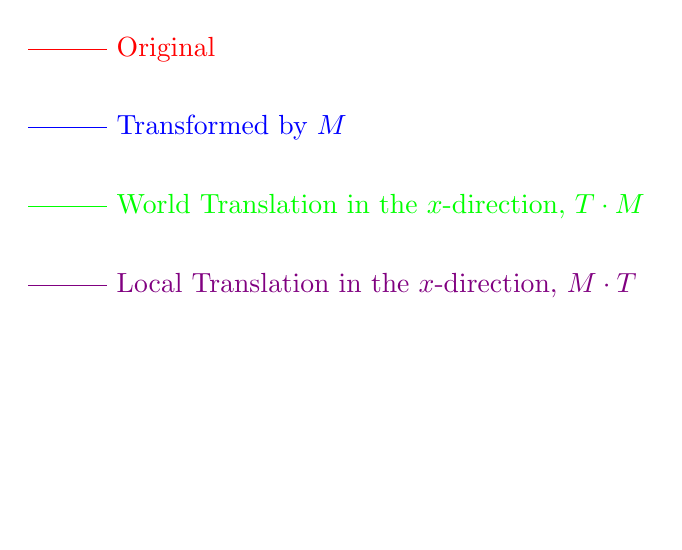
\begin{tikzpicture}
	\draw [red] (0,0) -- (1,0) node [right] {Original};
	\draw [blue] (0,-1) -- (1,-1) node [right] {Transformed by $M$};
	\draw [green] (0,-2) -- (1,-2) node [right] {World Translation in the $x$-direction, $T \cdot M$};
	\draw [violet] (0,-3) -- (1,-3) node [right] {Local Translation in the $x$-direction, $M \cdot T$};
	\path (0,-6) circle (0pt);
\end{tikzpicture}


%%% Useful Blocks of Code
\begin{comment}
$\displaystyle
\left[
\begin{array}{cccc}
	
\end{array}
\right] 
$
\end{comment}













\section{Thursday 20 September:  OpenGL Architecture}

\subsection{More Homogeneous Transformation Matrices}

\subsubsection{Rotation about the $z$ axis }

(Derived in {\tt 0918.tex} notes)

Rotation in the $xy$ plane, taking points on the positive $x$-axis towards the positive $y$-axis.

\tdplotsetmaincoords{70}{110}
\hfil\begin{tikzpicture}[scale=1,tdplot_main_coords]

%set up some coordinates 
%-----------------------
\coordinate (O) at (0,0,0);
\coordinate (p1) at (0,1,0);
\coordinate (p2) at (4,1,0);
\coordinate (p3) at (4,2,0);
\coordinate (p4) at (6,0,0);
\draw [black, ultra thick] (O) -- (p1) -- (p2) -- (p3) -- (p4);

\draw[thick,->] (O) -- (8,0,0) node[anchor=north east]{$x$};
\draw[thick,->] (O) -- (0,3,0) node[anchor=north west]{$y$};
\draw[thick,->] (O) -- (0,0,1) node[anchor=east]{$z$};

	\tdplotsetrotatedcoords{0}{0}{30}
	\coordinate (Shift) at (0,0,0);
	\tdplotsetrotatedcoordsorigin{(Shift)}
	\draw[thick,color=blue,tdplot_rotated_coords,->] (0,0,0) --
        (8,0,0) node[anchor=north east]{$x'$};
	\draw[thick,color=blue,tdplot_rotated_coords,->] (0,0,0) --
        (0,3,0) node[anchor=west]{$y'$};
	\draw[thick,color=blue,tdplot_rotated_coords,->] (0,0,0) --
        (0,0,.5) node[anchor=east]{$z'$};
	\draw [thick, color=blue, -triangle 60] (1.5,0,0) arc (0:30:1.5) node [midway, below] {$\theta$};
	\draw [blue, ultra thick, tdplot_rotated_coords] (0,0,0) -- (0,1,0) -- (4,1,0) -- (4,2,0) -- (6,0,0);
\end{tikzpicture}


$$
\left[ 
	\begin{array}{cccc}
		\cos \theta & -\sin \theta\cr
		\sin \theta & \cos \theta  \cr
	\end{array}
\right]
$$

3D version:

$$
\left[ 
	\begin{array}{cccc}
		\cos \theta & -\sin \theta & 0 & 0 \cr
		\sin \theta & \cos \theta & 0 & 0 \cr
		0 & 0 & 1 & 0 \cr
		0 & 0 & 0 & 1 \cr
	\end{array}
\right]
$$

\subsubsection{Rotation about the $y$-axis}

Note that this transformation makes points on the positive $z$-axis rotate towards the positive $x$-axis.

\tdplotsetmaincoords{60}{120}
%
\pgfmathsetmacro{\rvec}{6}
\pgfmathsetmacro{\thetavec}{60}
\pgfmathsetmacro{\phivec}{0}
%
\hfil\begin{tikzpicture}[scale=1,tdplot_main_coords]
	\coordinate (O) at (0,0,0);
	\draw[thick,->] (0,0,0) -- (7,0,0) node[anchor=north east]{$x$};
	\draw[thick,->] (0,0,0) -- (0,4,0) node[anchor=north west]{$y$};
	\draw[thick,->] (0,0,0) -- (0,0,4) node[anchor=south]{$z$};

	\draw [black, ultra thick] (0,0,0) -- (0,1,0) -- (4,1,0) -- (4,2,0) -- (6,0,0);

	\tdplotsetthetaplanecoords{\phivec}
	\tdplotdrawarc[tdplot_rotated_coords,blue,-triangle 60]{(0,0,0)}{3}{0}{\thetavec}{anchor=south east}{$\theta$}
	\tdplotdrawarc[tdplot_rotated_coords,dashed]{(0,0,0)}{6}{90}{150}{}{}

	\coordinate (Shift) at (0,1,0);
	\tdplotsetrotatedcoordsorigin{(Shift)}
	\tdplotdrawarc[tdplot_rotated_coords,dashed]{(0,0,0)}{4}{90}{150}{}{}

	\coordinate (Shift2) at (0,2,0);
	\tdplotsetrotatedcoordsorigin{(Shift2)}
	\tdplotdrawarc[tdplot_rotated_coords,dashed]{(0,0,0)}{4}{90}{150}{}{}

	\coordinate (Shift3) at (0,0,0);
	\tdplotsetrotatedcoordsorigin{(Shift3)}
	\tdplotsetrotatedcoords{0}{60}{0}

	\draw [blue, ultra thick, tdplot_rotated_coords] (0,0,0) -- (0,1,0) -- (4,1,0) -- (4,2,0) -- (6,0,0);

	\draw[thick,color=blue,tdplot_rotated_coords,->] (0,0,0) --
        (7,0,0) node[anchor=north east]{$x'$};
	\draw[thick,color=blue,tdplot_rotated_coords,->] (0,0,0) --
        (0,3,0) node[anchor=south]{$y'$};
	\draw[thick,color=blue,tdplot_rotated_coords,->] (0,0,0) --
        (0,0,4) node[anchor=east]{$z'$};

\end{tikzpicture}

Take this rotation for the 2D $zx$ plane:

$$
\left[ 
	\begin{array}{cccc}
		\cos \theta & -\sin \theta\cr
		\sin \theta & \cos \theta  \cr
	\end{array}
\right]
$$

Think of the first column and first row of the 2D array as the $z$ things, and the second column and second row as the $x$ things, and put them in the corresponding places in the 3D array.  

$$
\left[ 
	\begin{array}{cccc}
		\cos \theta & 0 & \sin \theta & 0 \cr
		0 & 1 & 0 & 0 \cr
		-\sin \theta & 0 & \cos \theta & 0 \cr
		0 & 0 & 0 & 1 \cr
	\end{array}
\right]
$$

\subsubsection{Rotation about the $x$-axis (Brad's Guess)}

Note that this transformation makes points on the positive $z$-axis rotate towards the positive $x$-axis.

\tdplotsetmaincoords{60}{120}
%
\pgfmathsetmacro{\rvec}{6}
\pgfmathsetmacro{\thetavec}{60}
\pgfmathsetmacro{\phivec}{90}
%
\hfil\begin{tikzpicture}[scale=1,tdplot_main_coords]
	\coordinate (O) at (0,0,0);
	\draw[thick,->] (0,0,0) -- (7,0,0) node[anchor=south]{$x$};
	\draw[thick,->] (0,0,0) -- (0,4,0) node[anchor=north west]{$y$};
	\draw[thick,->] (0,0,0) -- (0,0,5) node[anchor=south]{$z$};

	\draw [black, ultra thick] (0,0,0) -- (0,1,0) -- (4,1,0) -- (4,2,0) -- (6,0,0);

%	\tdplotsetthetaplanecoords{\phivec}
%	\tdplotdrawarc[tdplot_rotated_coords,blue,-triangle 60]{(0,0,0)}{3}{0}{\thetavec}{anchor=south east}{$\theta$}
%	\tdplotdrawarc[tdplot_rotated_coords,dashed]{(0,0,0)}{6}{90}{150}{}{}

%	\coordinate (Shift) at (0,1,0);
%	\tdplotsetrotatedcoordsorigin{(Shift)}
%	\tdplotdrawarc[tdplot_rotated_coords,dashed]{(0,0,0)}{4}{90}{150}{}{}

%	\coordinate (Shift2) at (0,2,0);
%	\tdplotsetrotatedcoordsorigin{(Shift2)}
%	\tdplotdrawarc[tdplot_rotated_coords,dashed]{(0,0,0)}{4}{90}{150}{}{}

%	\coordinate (Shift3) at (0,0,0);
%	\tdplotsetrotatedcoordsorigin{(Shift3)}

	\tdplotsetrotatedcoords{90}{{360-80}}{270}
	\draw [blue, ultra thick, tdplot_rotated_coords] (0,0,0) -- (0,1,0) -- (4,1,0) -- (4,2,0) -- (6,0,0);
	\draw[thick,color=blue,tdplot_rotated_coords,->] (0,0,0) -- (8,0,0) node[anchor=south]{$x'$};
	\draw[thick,color=blue,tdplot_rotated_coords,->] (0,0,0) -- (0,3,0) node[anchor=south]{$y'$};
	\draw[thick,color=blue,tdplot_rotated_coords,->] (0,0,0) -- (0,0,4) node[anchor=east]{$z'$};


\end{tikzpicture}



Take this rotation in the 2D $yz$ plane:

$$
\left[ 
	\begin{array}{cccc}
		\cos \theta & -\sin \theta\cr
		\sin \theta & \cos \theta  \cr
	\end{array}
\right]
$$

Think of the first column and first row of the 2D array as the $y$ things, and the second column and second row as the $z$ things, and put them in the corresponding places in the 3D array.  

$$
\left[ 
	\begin{array}{cccc}
		1 & 0 & 0 & 0 \cr
		0 & \cos \theta & -\sin \theta & 0 \cr
		0 & \sin \theta & \cos \theta & 0 \cr
		0 & 0 & 0 & 1 \cr
	\end{array}
\right]
$$

\subsubsection{Shear Example}

Notation:  $sh_x$ is ``shear factor.''

\

$$
\left[
	\begin{array}{cccc}
		x' \cr y' \cr z' \cr 1 \cr
	\end{array}
\right]
=
\left[
	\begin{array}{cccc}
		1 & sh_x & 0 & 0 \cr
		0 & 1 & 0 & 0 \cr
		0 & sh_z & 1 & 0 \cr
		0 & 0 & 0 & 1 \cr
	\end{array}
\right]
\left[
	\begin{array}{cccc}
		x \cr y \cr z \cr 1 \cr
	\end{array}
\right]
=
\left[
	\begin{array}{cccc}
		x + sh_x  y\cr
		y \cr
		z + sh_z y  \cr
		1 \cr
	\end{array}
\right]
$$

\


\begin{figure}
\centering

\tdplotsetmaincoords{60}{120}
%
\pgfmathsetmacro{\rvec}{6}
\pgfmathsetmacro{\thetavec}{60}
\pgfmathsetmacro{\phivec}{90}
%
\hfil\begin{tikzpicture}[scale=5,tdplot_main_coords]
	\coordinate (O) at (0,0,0);
	\draw[thick,->] (0,0,0) -- (1.5,0,0) node[anchor=south]{$x$};
	\draw[thick,->] (0,0,0) -- (0,1.5,0) node[anchor=north west]{$y$};
	\draw[thick,->] (0,0,0) -- (0,0,1.5) node[anchor=south]{$z$};

	\draw [black, ultra thick] (0,0,0) -- (0,1,0) -- (0,1,1) -- (0,0,1) -- (0,0,0);
	\draw [black, ultra thick] (1,0,0) -- (1,1,0) -- (1,1,1) -- (1,0,1) -- (1,0,0);
	\draw [black, ultra thick] (0,0,0) -- (1,0,0);
	\draw [black, ultra thick] (0,0,1) -- (1,0,1);
	\draw [black, ultra thick] (0,1,0) -- (1,1,0);
	\draw [black, ultra thick] (0,1,1) -- (1,1,1);

%	\draw [blue, ultra thick] (0,0,0) -- (0,1,0) -- (0,1,1) -- (0,0,1) -- (0,0,0);
%	\draw [blue, ultra thick] (1,0,0) -- (1,1,0) -- (1,1,1) -- (1,0,1) -- (1,0,0);
%	\draw [blue, ultra thick] (0,0,0) -- (1,0,0);
%	\draw [blue, ultra thick] (0,0,1) -- (1,0,1);
%	\draw [blue, ultra thick] (0,1,0) -- (1,1,0);
%	\draw [blue, ultra thick] (0,1,1) -- (1,1,1);

	\draw [blue, ultra thick] (0,0,0) -- (0.5,1,-0.5) -- (0.5,1,0.5) -- (0,0,1) -- (0,0,0);
	\draw [blue, ultra thick] (1,0,0) -- (1.5,1,-0.5) -- (1.5,1,0.5) -- (1,0,1) -- (1,0,0);
	\draw [blue, ultra thick] (0,0,0) -- (1,0,0);
	\draw [blue, ultra thick] (0,0,1) -- (1,0,1);
	\draw [blue, ultra thick] (0.5,1,-0.5) -- (1.5,1,-0.5);
	\draw [blue, ultra thick] (0.5,1,0.5) -- (1.5,1,0.5);



\end{tikzpicture}
\caption{Shear with $sh_x = 0.5$ and $sh_z = -0.5$.} \label{fig:M1}
\end{figure}



\subsubsection{Composition Example}

Rotate by $\theta$  about $z$-direction vector through a pivot point, $P$.   

1.  Translate by $\displaystyle -P \ = 
\left[ 
	\begin{array}{c}
		-p_x \cr
		-p_y \cr
		-p_z \cr
		1 \cr
	\end{array}
\right]
$.

2.  Rotate about $z$-axis.

3.  Translate back by $P$.  

\

$$
	\left[
		\begin{array}{cccc}
			x' \cr y' \cr z' \cr 1 \cr
		\end{array}
	\right]
=
	\left[
		\begin{array}{cccc}
			1 & 0 & 0 & p_x \cr
			0 & 1 & 0 & p_y \cr
			0 & 0 & 1 & p_z \cr
			0 & 0 & 0 & 1 \cr
		\end{array}
	\right]
	\left[
		\begin{array}{cccc}
			\cos \theta & -\sin \theta & 0 & 0 \cr
			\sin \theta & \cos \theta & 0 & 0 \cr
			0 & 0 & 1 & 0 \cr
			0 & 0 & 0 & 1 \cr
		\end{array}
	\right]
	\left[
		\begin{array}{cccc}
			1 & 0 & 0 & -p_x \cr
			0 & 1 & 0 & -p_y \cr
			0 & 0 & 1 & -p_z \cr
			0 & 0 & 0 & 1 \cr
		\end{array}
	\right]
	\left[
		\begin{array}{cccc}
			x  \cr
			y \cr
			z \cr
			1
		\end{array}
	\right]
$$


\subsection{OpenGL Architecture}

Simplified OpenGL Architecture

\

{\it Vertex Array Object} is the mesh data, storage

\qquad $\Downarrow$

{\it Vertex Shader} transforms the vertices, sets up attributes for interpolation


\qquad $\Downarrow$

[Other Shaders]

\qquad $\Downarrow$


{\it Rasterizer} does scan conversion with interpolated attributes

\qquad $\Downarrow$


{\it Fragment Shader} Assigns colors, typically based on lighting equation.  
A {\it fragment} is a pixel with additional information.

\qquad $\Downarrow$


{\it Frame Buffer}

\

Note that, by default, OpenGL has coordinates in $[-1,1]$.

\

Read OpenGL book about {\it primitive restart}.



\section{Euler Angles, Euler Rotations}

Euler angles (rotations) are expressed in Ti\textit{k}Z-3dplot as $(\alpha, \beta, \gamma)$.   

The black coordinate system (world) is rotated about the $z$-axis by $\alpha$ to become the blue coordinate system.  

Then the blue coordinate system is rotated about the new $y$-axis by $\beta$ to become the red coordinate system.

Then the red coordinate system is rotated about the new $z$-axis by $\gamma$ become the purple coordinate system.


\tdplotsetmaincoords{60}{120}
%
\pgfmathsetmacro{\rvec}{6}
\pgfmathsetmacro{\thetavec}{60}
\pgfmathsetmacro{\phivec}{90}
%
\begin{tikzpicture}[scale=1,tdplot_main_coords]
	\coordinate (O) at (0,0,0);
	\draw[thick,->] (0,0,0) -- (7,0,0) node[anchor=north east]{$x$};
	\draw[thick,->] (0,0,0) -- (0,4,0) node[anchor=north west]{$y$};
	\draw[thick,->] (0,0,0) -- (0,0,5) node[anchor=south]{$z$};

	\draw [black, ultra thick] (0,0,0) -- (0,1,0) -- (4,1,0) -- (4,2,0) -- (6,0,0);

%	\tdplotsetthetaplanecoords{\phivec}
%	\tdplotdrawarc[tdplot_rotated_coords,blue,-triangle 60]{(0,0,0)}{3}{0}{\thetavec}{anchor=south east}{$\theta$}
%	\tdplotdrawarc[tdplot_rotated_coords,dashed]{(0,0,0)}{6}{90}{150}{}{}

%	\coordinate (Shift) at (0,1,0);
%	\tdplotsetrotatedcoordsorigin{(Shift)}
%	\tdplotdrawarc[tdplot_rotated_coords,dashed]{(0,0,0)}{4}{90}{150}{}{}

%	\coordinate (Shift2) at (0,2,0);
%	\tdplotsetrotatedcoordsorigin{(Shift2)}
%	\tdplotdrawarc[tdplot_rotated_coords,dashed]{(0,0,0)}{4}{90}{150}{}{}

%	\coordinate (Shift3) at (0,0,0);
%	\tdplotsetrotatedcoordsorigin{(Shift3)}
	\tdplotsetrotatedcoords{10}{0}{0}
	\draw [blue, ultra thick, tdplot_rotated_coords] (0,0,0) -- (0,1,0) -- (4,1,0) -- (4,2,0) -- (6,0,0);
	\draw[thick,color=blue,tdplot_rotated_coords,->] (0,0,0) -- (7,0,0) node[anchor=north east]{$x'$};
	\draw[thick,color=blue,tdplot_rotated_coords,->] (0,0,0) -- (0,3,0) node[anchor=south]{$y'$};
	\draw[thick,color=blue,tdplot_rotated_coords,->] (0,0,0) -- (0,0,4) node[anchor=east]{$z'$};

	\tdplotsetrotatedcoords{10}{20}{0}
	\draw [red, ultra thick, tdplot_rotated_coords] (0,0,0) -- (0,1,0) -- (4,1,0) -- (4,2,0) -- (6,0,0);
	\draw[thick,color=red,tdplot_rotated_coords,->] (0,0,0) -- (7,0,0) node[anchor=north east]{$x''$};
	\draw[thick,color=red,tdplot_rotated_coords,->] (0,0,0) -- (0,2,0) node[anchor=south]{$y''$};
	\draw[thick,color=red,tdplot_rotated_coords,->] (0,0,0) -- (0,0,4) node[anchor=east]{$z''$};

	\tdplotsetrotatedcoords{10}{20}{20}
	\draw [violet, ultra thick, tdplot_rotated_coords] (0,0,0) -- (0,1,0) -- (4,1,0) -- (4,2,0) -- (6,0,0);
	\draw[thick,color=violet,tdplot_rotated_coords,->] (0,0,0) -- (7,0,0) node[anchor=north east]{$x'''$};
	\draw[thick,color=violet,tdplot_rotated_coords,->] (0,0,0) -- (0,2,0) node[anchor=south]{$y'''$};
	\draw[thick,color=violet,tdplot_rotated_coords,->] (0,0,0) -- (0,0,3) node[anchor=east]{$z'''$};

\end{tikzpicture}


\section{Assignment \#2 on  a Mac/Linux Box}

1.  Put the {\tt gmtl} folder in your {\tt /usr/local/include} directory.  

\

2.  Somehow, some of the {\tt \#include} statements repeat.  I don't know if that's a problem, but take the repetition out.  

\begin{verbatim}
#include <stdlib.h>
#include <stdio.h>


#include <gmtl\gmtl.h>
#include <stdlib.h>
#include <stdio.h>
\end{verbatim}

3.  Line 9:  Change 

\begin{verbatim}#include <GL/glew.h>\end{verbatim} 

to  

\begin{verbatim}#include <GL\glew.h>\end{verbatim}

4.  In line 24, the {\tt fopen\_s} will give you trouble.  

\begin{verbatim}
	fopen_s(&fptr, file, "rb");	
\end{verbatim}


All of the {\tt *\_s} stuff is new to the C11 standard, which is not widely supported.  Since it only appears once, you could rewrite that line as:

\begin{verbatim}
	fptr = fopen ( file, "rb");
\end{verbatim}

If some function like this occurs a lot, you could redefine it near the top of your file:

\begin{verbatim}
#ifdef __APPLE__
    #define fopen_s(pFile,filename,mode) ((*(pFile))=fopen((filename),(mode)))==NULL
#endif
\end{verbatim}


\

5.  As we did in the very first assignment, uncomment/add these lines at line 58:

\begin{verbatim}
    glfwWindowHint(GLFW_CONTEXT_VERSION_MAJOR, 3);
    glfwWindowHint(GLFW_CONTEXT_VERSION_MINOR, 3);
    glfwWindowHint(GLFW_OPENGL_FORWARD_COMPAT, GL_TRUE);
    glfwWindowHint(GLFW_OPENGL_PROFILE, GLFW_OPENGL_CORE_PROFILE);
\end{verbatim}

\

6.  As Lou mentioned in her forum post, in the {\tt OpenGL\_Example.frag} file, the {\tt gl\_FragColor} should be a dummy variable, but actually means something.  In lines 3 and 7, change both of them to the same thing.  I called them ``Fred.''

\

7.  I compiled with these flags and libraries.  

\begin{verbatim}
$ g++ C00412257_Assignment_02.cpp -framework OpenGL -lGLEW -lGLFW -w
\end{verbatim}





%%%%%%%%%%%%%
%
% End Stuff
%
%%%%%%%%%

\end{spacing}
\end{document}

%%%%%%%%%%%
%
% Useful code to recycle
%
%%%%%%%%%%

\hfil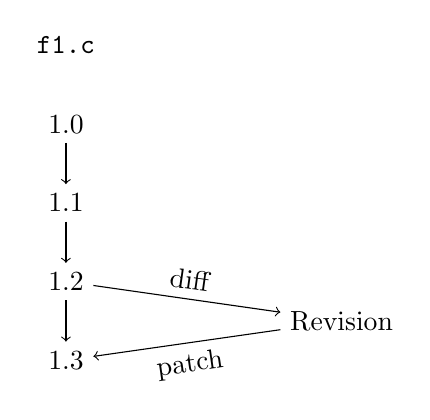
\begin{tikzpicture}
	[scale=0.5]
	\node (n0) at (0,0) {\tt f1.c};
	\node (n1) at (0,-2)  {1.0};
	\node (n2) at (0,-4)  {1.1};
	\node (n3) at (0,-6)  {1.2};
	\node (n4) at (0,-8)  {1.3};
	\node (n7) at (7,-7) {Revision};
  
	\foreach \from/\to in {n1/n2,n2/n3,n3/n4}
	\draw [->] (\from) -- (\to);

	\draw [->] (n3) -- node [above, sloped, midway] {diff} (n7);
	\draw [<-] (n4) -- node [below, sloped, midway] {patch} (n7);
\end{tikzpicture}









































